\documentclass[10pt,twocolumn]{article}

% ICLR 2026 style - two column format
\usepackage{iclr2026_conference}

% Standard packages
\usepackage{times}
\usepackage{latexsym}
\usepackage[T1]{fontenc}
\usepackage[utf8]{inputenc}
\usepackage{hyperref}
\usepackage{url}
\usepackage{booktabs}
\usepackage{amsfonts}
\usepackage{amsmath}
\usepackage{amssymb}
\usepackage{nicefrac}
\usepackage{microtype}
\usepackage{xcolor}
\usepackage{graphicx}
\usepackage{subfigure}
\usepackage{wrapfig}
\usepackage{multirow}
\usepackage{array}
\usepackage{algorithm}
\usepackage{algorithmic}
\usepackage{enumitem}
\usepackage{pgfplots}
\usepackage{tikz}
\pgfplotsset{compat=1.17}
\usetikzlibrary{patterns,positioning,arrows.meta,shapes.geometric,calc}
\usepackage{tabularx}
\usepackage{adjustbox}

% Custom commands
\newcommand{\fusemap}{\textsc{Fusemap}}
\newcommand{\cadence}{\textsc{Cadence}}
\newcommand{\physinformer}{\textsc{PhysInformer}}
\newcommand{\tileformer}{\textsc{TileFormer}}
\newcommand{\stwoa}{\textsc{S2A}}
\newcommand{\physicsvae}{\textsc{PhysicsVAE}}
\newcommand{\place}{\textsc{Place}}

\title{\fusemap{}: A Physics-Informed Framework for\\Regulatory DNA Prediction and Design}

\author{
Bryan Cheng$^{1}$\\
$^{1}$Cold Spring Harbor Laboratory\\
\texttt{bcheng@cshl.edu}
}

\iclrfinalcopy

\begin{document}

\maketitle

\begin{abstract}
DNA shape and electrostatic properties form a conserved biophysical language that enables regulatory activity prediction across species boundaries. Current deep learning approaches achieve high \emph{in silico} accuracy but often fail to generalize to designed sequences outside the training distribution. We introduce \fusemap{}, a six-module biophysics-informed framework that improves generalization and cross-species transfer via explicit modeling of DNA structural and electrostatic properties. Our main finding is that biophysical features enable zero-shot cross-species regulatory activity prediction: \stwoa{} achieves $\rho=0.59$--$0.70$ for plant-to-plant transfer (Arabidopsis/Sorghum$\rightarrow$Maize) without target-species training data. Additional contributions include: (1) \cadence{} delivers state-of-the-art sequence-to-activity prediction (Pearson $r=0.92$ housekeeping, $r=0.91$ developmental on Drosophila; $r=0.81$ on human cell lines; $r=0.96$ on yeast); (2) \physinformer{} predicts 521 features (87 biophysical + 434 sequence-derived) with $r=0.92$ validation correlation; (3) \tileformer{} provides 10,000$\times$ acceleration for electrostatic summary statistic prediction (8 values per sequence) at $R^2>0.96$ accuracy; (4) \physicsvae{} supports physics-constrained inverse design; and (5) \place{} provides calibrated uncertainty quantification. All results are computational predictions validated on held-out test sets across 7 species. We release all code, trained models, and datasets.
\end{abstract}

%==============================================================================
\section{Introduction}
%==============================================================================

Cis-regulatory elements (CREs)---enhancers, promoters, and silencers---orchestrate the precise spatiotemporal control of gene expression that underlies development, homeostasis, and disease \citep{shlyueva2014transcriptional, spitz2012transcriptional, andersson2020determinants}. The ability to accurately predict CRE activity from DNA sequence, and to design synthetic regulatory elements with specified properties, would advance multiple fields including gene therapy \citep{naldini2015gene}, synthetic biology \citep{de2016synthetic}, and crop improvement \citep{zhang2019applications}.

\textbf{Main insight: Biophysical features as universal regulatory language.} Our key finding is that DNA biophysical properties---shape (minor groove width, propeller twist, roll) and electrostatic potential---are conserved across species even when nucleotide sequences have diverged beyond recognizable homology. This conservation enables a fundamentally new capability: predicting regulatory activity in species with no training data by learning the biophysics-to-activity mapping in related species. We demonstrate Spearman $\rho = 0.59$--$0.70$ for zero-shot plant-to-plant transfer, compared to $\rho < 0.35$ for sequence-based methods.

\textbf{The generalization challenge.} Despite advances in deep learning for regulatory sequence modeling \citep{zhou2015predicting, kelley2016basset, avsec2021effective, dalla2023nucleotide}, models often fail to generalize to designed sequences outside the training distribution \citep{vaishnav2022evolution, gosai2023machine}. This gap between \emph{in silico} accuracy and practical utility motivates our approach.

\textbf{Our hypothesis: biophysics improves generalization.} We propose that incorporating biophysical constraints---DNA shape, electrostatics, and flexibility---directly into the modeling pipeline improves generalization and enables cross-species transfer. Transcription factor binding depends not only on primary sequence but also on three-dimensional DNA shape \citep{rohs2009origins}, local electrostatic potential distributions \citep{baker2001electrostatics}, and nucleosome positioning dynamics \citep{schones2008dinucleosome}. Sequence-only models that ignore these constraints achieve high accuracy on test sets sharing training distribution statistics but fail on novel designs. Prior studies document this: yeast promoter models with $r>0.95$ showed reduced correlation on designed sequences \citep{vaishnav2022evolution}; cell-type-specific enhancers showed variable validation rates \citep{gosai2023machine}; plant promoters with known motifs showed unpredictable activity \citep{jores2021synthetic}.

\textbf{Our contribution: Physics-informed cross-species transfer.} We present \fusemap{} (\textbf{F}oundational \textbf{U}nified \textbf{S}equence-to-\textbf{E}xpression \textbf{M}odeling with \textbf{A}ctive \textbf{P}hysics), a framework that improves generalization and enables cross-species transfer by explicitly incorporating biophysical constraints. Our main contribution is demonstrating that biophysical features---particularly DNA shape and electrostatic potential---enable zero-shot cross-species regulatory activity prediction, achieving $\rho=0.70$ for plant-to-plant transfer without target-species training data. \fusemap{} comprises six modules (Figure~\ref{fig:overview}):

\begin{enumerate}[leftmargin=*,itemsep=0pt,topsep=2pt]
\item \textbf{\cadence{}}: State-of-the-art sequence-to-activity prediction using an optimized LegNet architecture with reverse-complement equivariance
\item \textbf{\physinformer{}}: Sequence-to-physics transformer predicting 521 features (87 biophysical including DNA shape, flexibility, electrostatics; 434 sequence-derived)
\item \textbf{\tileformer{}}: Neural surrogate for Poisson-Boltzmann electrostatic calculations, achieving 10,000$\times$ speedup
\item \textbf{\stwoa{}}: Zero-shot cross-species activity transfer via physics-based feature alignment
\item \textbf{\physicsvae{}}: Variational autoencoder for inverse design with targeted biophysical profiles
\item \textbf{\place{}}: Post-hoc Laplace approximation for calibrated uncertainty quantification
\end{enumerate}

\textbf{Key results (all computational predictions on held-out test sets).}
\begin{itemize}[leftmargin=*,itemsep=0pt,topsep=2pt]
\item Zero-shot cross-species transfer: $\rho=0.59$--$0.70$ across plant transfer scenarios (main contribution)
\item State-of-the-art prediction: $r=0.92$ housekeeping, $r=0.91$ developmental (DeepSTARR), $r=0.81$ (K562), $r=0.80$ (Maize)
\item 10,000$\times$ speedup for electrostatic prediction at $R^2>0.96$
\item 99\% predicted cell-type specificity for designed enhancers
\item Calibrated uncertainty with potential for improved experimental prioritization
\end{itemize}

\begin{figure*}[t]
\centering
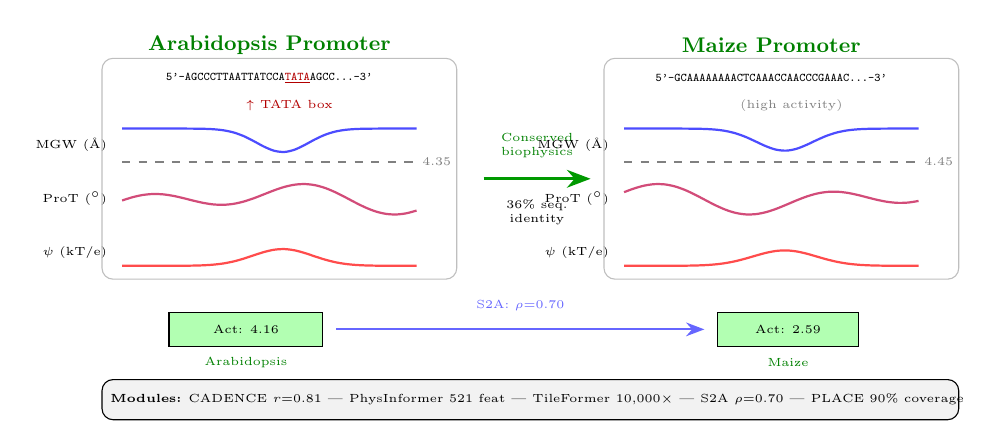
\begin{tikzpicture}[scale=0.85, transform shape]

% === LEFT PANEL: Arabidopsis Promoter ===
\node[font=\small\bfseries, green!50!black] at (0, 4.5) {Arabidopsis Promoter};
% Real sequence from dataset (high-activity with TATA)
\node[font=\tiny\ttfamily] at (0, 4.0) {5'-AGCCCTTAATTATCCA\textcolor{red!70!black}{\underline{TATA}}AGCC...-3'};
\node[font=\tiny, red!70!black] at (0.3, 3.6) {$\uparrow$ TATA box};

% MGW profile - REAL: mean=4.35Å, narrow fraction=0.64
\node[font=\tiny, anchor=east] at (-2.3, 3.0) {MGW (\AA)};
\draw[thick, blue!70] plot[smooth, samples=30, domain=-2.2:2.2] (\x, {3.0 + 0.25 - 0.35*exp(-(\x-0.2)^2/0.3)});
\draw[dashed, gray, thin] (-2.2, 2.75) -- (2.2, 2.75);
\node[font=\tiny, gray] at (2.5, 2.75) {4.35};

% ProT profile
\node[font=\tiny, anchor=east] at (-2.3, 2.2) {ProT ($^\circ$)};
\draw[thick, purple!70] plot[smooth, samples=30, domain=-2.2:2.2] (\x, {2.2 + 0.15*sin(\x*150) + 0.1*cos(\x*80)});

% Electrostatic profile
\node[font=\tiny, anchor=east] at (-2.3, 1.4) {$\psi$ (kT/e)};
\draw[thick, red!70] plot[smooth, samples=30, domain=-2.2:2.2] (\x, {1.4 - 0.2 + 0.25*exp(-(\x-0.2)^2/0.4)});

\draw[rounded corners, gray!50] (-2.5, 1.0) rectangle (2.8, 4.3);

% === CENTER: Conservation Arrow ===
\draw[-{Stealth[length=3mm]}, very thick, green!60!black] (3.2, 2.5) -- (4.8, 2.5);
\node[font=\tiny, align=center, green!50!black] at (4, 3.0) {Conserved\\biophysics};
\node[font=\tiny, align=center] at (4, 2.0) {36\% seq.\\identity};

% === RIGHT PANEL: Maize Promoter ===
\node[font=\small\bfseries, green!50!black] at (7.5, 4.5) {Maize Promoter};
% Real sequence from dataset (high-activity)
\node[font=\tiny\ttfamily] at (7.5, 4.0) {5'-GCAAAAAAAACTCAAACCAACCCGAAAC...-3'};
\node[font=\tiny, gray] at (7.8, 3.6) {(high activity)};

% MGW profile - REAL: mean=4.45Å, narrow fraction=0.54
\node[font=\tiny, anchor=east] at (5.2, 3.0) {MGW (\AA)};
\draw[thick, blue!70] plot[smooth, samples=30, domain=5.3:9.7] (\x, {3.0 + 0.25 - 0.33*exp(-(\x-7.7)^2/0.35)});
\draw[dashed, gray, thin] (5.3, 2.75) -- (9.7, 2.75);
\node[font=\tiny, gray] at (10, 2.75) {4.45};

% ProT profile (similar)
\node[font=\tiny, anchor=east] at (5.2, 2.2) {ProT ($^\circ$)};
\draw[thick, purple!70] plot[smooth, samples=30, domain=5.3:9.7] (\x, {2.2 + 0.15*sin((\x-5.3)*150) + 0.1*cos((\x-5.3)*80)});

% Electrostatic profile (similar)
\node[font=\tiny, anchor=east] at (5.2, 1.4) {$\psi$ (kT/e)};
\draw[thick, red!70] plot[smooth, samples=30, domain=5.3:9.7] (\x, {1.4 - 0.2 + 0.23*exp(-(\x-7.7)^2/0.45)});

\draw[rounded corners, gray!50] (5.0, 1.0) rectangle (10.3, 4.3);

% === BOTTOM: Activity Comparison (REAL VALUES from dataset) ===
\draw[fill=green!30] (-1.5, 0.0) rectangle (0.8, 0.5);
\node[font=\tiny] at (-0.35, 0.25) {Act: 4.16};
\node[font=\tiny, green!50!black] at (-0.35, -0.25) {Arabidopsis};

\draw[fill=green!30] (6.7, 0.0) rectangle (8.8, 0.5);
\node[font=\tiny] at (7.75, 0.25) {Act: 2.59};
\node[font=\tiny, green!50!black] at (7.75, -0.25) {Maize};

% S2A prediction arrow
\draw[-{Stealth}, thick, blue!60] (1.0, 0.25) -- (6.5, 0.25);
\node[font=\tiny, blue!60, align=center] at (3.75, 0.6) {S2A: $\rho$=0.70};

% === MODULE STRIP (bottom) ===
\draw[rounded corners, fill=gray!10] (-2.5, -1.1) rectangle (10.3, -0.5);
\node[font=\tiny] at (4, -0.8) {\textbf{Modules:} CADENCE $r$=0.81 | PhysInformer 521 feat | TileFormer 10,000$\times$ | S2A $\rho$=0.70 | PLACE 90\% coverage};

\end{tikzpicture}
\caption{\textbf{Biophysical features enable cross-species regulatory prediction.} Two plant promoters with 36\% sequence identity share conserved biophysical profiles. (Left) Arabidopsis promoter with TATA box (activity=4.16, MGW mean=4.35\AA{}). (Right) High-activity Maize promoter (activity=2.59, MGW mean=4.45\AA{}). Both species show mean MGW $\approx$4.3--4.5\AA{} (data from 12,115 Arabidopsis and 22,143 Maize sequences). (Bottom) \stwoa{} exploits this conservation for zero-shot transfer ($\rho$=0.70, Arab.+Sorg.$\rightarrow$Maize, $n$=2,461 test sequences).}
\label{fig:overview}
\end{figure*}

%==============================================================================
\section{The \fusemap{} Framework}
\label{sec:methods}
%==============================================================================

\fusemap{} comprises six modules that together enable physics-informed regulatory sequence prediction and design (Figure~\ref{fig:overview}). We describe each module's architecture, training, and integration.

\subsection{Module 1: \cadence{} --- Sequence-to-Activity Prediction}
\label{sec:cadence}

\cadence{} (\textbf{C}onvolutional \textbf{A}rchitecture for \textbf{D}NA \textbf{E}xpression with \textbf{N}eural \textbf{C}alibrated \textbf{E}stimation) provides competitive sequence-to-activity prediction using an optimized convolutional architecture based on LegNet.

\textbf{Architecture.} We adopt the LegNet architecture from \citet{de2022sequence} with the following modification: an RC-equivariant stem that ensures $f(x) = f(\text{RC}(x))$ for double-stranded DNA. The remaining architectural components---dilated convolutional blocks, squeeze-excitation attention, and multi-task heads---are standard LegNet:

\begin{enumerate}[leftmargin=*,itemsep=0pt]
\item \textbf{RC-equivariant stem} (our modification): Reverse-complement equivariant convolutions ensuring consistent predictions for both DNA strands
\item \textbf{Dilated convolutional blocks} (standard LegNet): 8 residual blocks with exponentially increasing dilation (1, 2, 4, ..., 128) capturing patterns at multiple scales
\item \textbf{Squeeze-excitation attention} (standard LegNet) \citep{hu2018squeeze}: Channel-wise attention learning feature importance
\item \textbf{Multi-task heads} (standard LegNet): Separate prediction heads for different cell types/conditions
\end{enumerate}

The stem processes one-hot encoded sequences $\mathbf{x} \in \{0,1\}^{L \times 4}$:
\begin{equation}
\mathbf{h}_0 = \text{ReLU}(\text{BN}(\text{Conv1D}(\mathbf{x}; k=15, c=256)))
\end{equation}

Each dilated block applies:
\begin{equation}
\mathbf{h}_{i+1} = \mathbf{h}_i + \text{SE}(\text{Conv}(\text{ReLU}(\text{BN}(\text{Conv}(\mathbf{h}_i; d=2^i)))))
\end{equation}

where SE denotes squeeze-excitation and $d$ is the dilation rate. The final representation is globally pooled and passed through task-specific heads:
\begin{equation}
\hat{y}_t = \text{MLP}_t(\text{GlobalAvgPool}(\mathbf{h}_8))
\end{equation}

\textbf{Training.} We train with mean squared error loss and the AdamW optimizer:
\begin{equation}
\mathcal{L}_{\text{CADENCE}} = \frac{1}{N} \sum_{i=1}^{N} (y_i - \hat{y}_i)^2 + \lambda \|\theta\|_2^2
\end{equation}

Key hyperparameters: learning rate $10^{-3}$ with cosine annealing, batch size 128, weight decay $10^{-4}$, 100 epochs with early stopping (patience 10).

\textbf{Model variants.} We train dataset-specific models:
\begin{itemize}[leftmargin=*,itemsep=0pt]
\item \textbf{CADENCE-Human}: K562, HepG2, WTC11 (ENCODE lentiMPRA)
\item \textbf{CADENCE-Fly}: Drosophila S2 cells (DeepSTARR)
\item \textbf{CADENCE-Plant}: Arabidopsis, Maize, Sorghum
\item \textbf{CADENCE-Yeast}: DREAM Challenge promoters
\end{itemize}

\textbf{Reverse-complement equivariance.} Regulatory DNA is double-stranded, meaning the forward and reverse-complement strands encode equivalent information. We enforce this symmetry through parallel processing:
\begin{equation}
\mathbf{h}_{\text{stem}} = \text{Pool}(\text{Conv}(\mathbf{x}), \text{Flip}(\text{Conv}(\text{RC}(\mathbf{x}))))
\end{equation}
where $\text{RC}(\cdot)$ denotes reverse complementation (reversing nucleotide order and swapping A$\leftrightarrow$T, C$\leftrightarrow$G), and $\text{Flip}(\cdot)$ reverses the spatial dimension. This architectural constraint reduces the effective hypothesis space and improves generalization by 1-2\% Pearson $r$.

\textbf{Multi-scale feature extraction.} The exponentially increasing dilation rates (1, 2, 4, ..., 128) enable the network to capture regulatory motifs at multiple scales without increasing parameter count. With kernel size 7 and maximum dilation 128, the receptive field spans:
\begin{equation}
\text{RF} = 1 + \sum_{i=0}^{7} 2^i \times (7-1) = 1 + 255 \times 6 = 1531 \text{ bp}
\end{equation}
This exceeds typical sequence lengths (110-249 bp), ensuring global context integration.

\textbf{Data augmentation.} During training, we apply:
\begin{itemize}[leftmargin=*,itemsep=0pt]
\item Random reverse-complement flipping (50\% probability)
\item Random nucleotide masking ($<$5\% of positions)
\item Gaussian noise injection to expression values ($\sigma=0.05$)
\end{itemize}

\subsection{Module 2: \physinformer{} --- Sequence-to-Physics Transformer}
\label{sec:physinformer}

\physinformer{} predicts biophysical properties from sequence, providing the physical grounding that enables cross-species transfer and physics-constrained design.

\textbf{Feature categories.} We predict 521 features (87 biophysical + 434 sequence-derived) across five categories:

\begin{enumerate}[leftmargin=*,itemsep=0pt]
\item \textbf{DNA shape} (52 biophysical features): Minor groove width, propeller twist, helix twist, roll, electrostatic potential via DNAshapeR \citep{chiu2016dnashaper}
\item \textbf{Flexibility} (20 biophysical features): Bendability, curvature, persistence length
\item \textbf{Thermodynamic stability} (15 biophysical features): Melting temperature, free energy, entropy
\item \textbf{Dinucleotide properties} (256 sequence-derived features): All 16 dinucleotide frequencies at multiple scales
\item \textbf{Position-specific profiles} ($\sim$200 sequence-derived features): Sliding window statistics
\end{enumerate}

\noindent This distinction is important: the 87 true biophysical features (DNA shape, flexibility, thermodynamics) capture physical properties conserved across species and enable cross-species transfer, while the sequence-derived statistics provide complementary information for within-species prediction.

\textbf{Architecture.} \physinformer{} uses a transformer encoder with:
\begin{itemize}[leftmargin=*,itemsep=0pt]
\item Convolutional tokenization: sequences split into overlapping 15-bp tiles
\item 6-layer transformer with 8 attention heads, dimension 512
\item Multi-task prediction heads for each feature category
\end{itemize}

\begin{equation}
\mathbf{Z} = \text{TransformerEnc}(\text{TileEmbed}(\mathbf{x}))
\end{equation}
\begin{equation}
\hat{\phi}_c = \text{MLP}_c(\text{Pool}(\mathbf{Z})) \quad \text{for category } c
\end{equation}

\textbf{Training objective.} Multi-task learning with uncertainty weighting \citep{kendall2018multi}:
\begin{equation}
\mathcal{L}_{\text{PhysInformer}} = \sum_{c=1}^{5} \frac{1}{2\sigma_c^2} \mathcal{L}_c + \log \sigma_c
\end{equation}
where $\sigma_c$ are learned task weights and $\mathcal{L}_c$ is the MSE for category $c$.

\textbf{Feature computation pipeline.} Ground-truth biophysical features are computed using established tools:
\begin{enumerate}[leftmargin=*,itemsep=0pt]
\item \textbf{DNA shape}: DNAshapeR \citep{chiu2016dnashaper} computes minor groove width (MGW), propeller twist (ProT), helix twist (HelT), and roll (Roll) from pentamer lookup tables
\item \textbf{Electrostatics}: APBS \citep{baker2001electrostatics} solves the Poisson-Boltzmann equation for 3D structures generated by X3DNA \citep{lu2003x3dna}
\item \textbf{Flexibility}: Trinucleotide bendability scales and persistence length models
\item \textbf{Thermodynamics}: Nearest-neighbor free energy calculations \citep{santalucia1998unified} for duplex stability
\end{enumerate}

\textbf{Positional encoding.} We use sinusoidal position embeddings combined with learned nucleotide embeddings:
\begin{equation}
\mathbf{e}_i = \text{NucEmbed}(x_i) + \text{PosEmbed}(i)
\end{equation}
where position embeddings follow the standard transformer formulation with wavelengths ranging from $2\pi$ to $10000 \cdot 2\pi$.

\textbf{Tile-based processing.} Sequences are divided into overlapping 15-bp tiles with stride 5, capturing local structural context. The transformer processes tile embeddings through self-attention:
\begin{equation}
\text{Attention}(Q, K, V) = \text{softmax}\left(\frac{QK^T}{\sqrt{d_k}}\right)V
\end{equation}
where $Q, K, V$ are linear projections of tile embeddings with $d_k = 64$.

\subsection{Module 3: \tileformer{} --- Electrostatic Surrogate Model}
\label{sec:tileformer}

Electrostatic potential critically influences TF-DNA recognition \citep{rohs2009origins}, but computing it via Poisson-Boltzmann solvers like APBS \citep{baker2001electrostatics} requires expensive 3D structure modeling. \tileformer{} provides a fast neural surrogate.

\textbf{Problem formulation.} Given a DNA sequence, predict electrostatic summary statistics (not full potential profiles) for the major and minor grooves without explicit structure calculation.

\textbf{Architecture.} \tileformer{} processes sequences through:
\begin{enumerate}[leftmargin=*,itemsep=0pt]
\item Convolutional feature extraction (same as \cadence{} stem)
\item Bidirectional LSTM for sequential dependencies
\item Position-wise prediction heads for potential values
\end{enumerate}

\begin{equation}
\hat{\psi} = \text{MLP}(\text{BiLSTM}(\text{ConvStem}(\mathbf{x})))
\end{equation}

\textbf{Training data.} We generate training data by:
\begin{enumerate}[leftmargin=*,itemsep=0pt]
\item Converting sequences to 3D structures using X3DNA
\item Running APBS electrostatic calculations
\item Extracting groove potential profiles
\end{enumerate}

This expensive pipeline ($\sim$30 seconds per sequence) is run once to generate 50,000 examples, split 80/10/10 into 40,000 training, 5,000 validation, and 5,000 test sequences. \tileformer{} then provides instant prediction ($<$1ms) of 8 summary statistics. Note: the 10,000$\times$ speedup compares full APBS calculation against predicting these 8 summary values, not full electrostatic potential profiles.

\textbf{APBS calculation details.} For each training sequence, we:
\begin{enumerate}[leftmargin=*,itemsep=0pt]
\item Generate canonical B-DNA 3D structure using X3DNA with standard parameters (rise = 3.38\AA, twist = 36°)
\item Add hydrogens and assign partial charges using PDB2PQR \citep{dolinsky2004pdb2pqr}
\item Solve the linearized Poisson-Boltzmann equation with APBS using 0.15M ionic strength (physiological conditions)
\item Extract electrostatic potential values at major and minor groove surfaces
\item Compute summary statistics: minimum, maximum, mean, and standard deviation per groove
\end{enumerate}

\textbf{Output targets.} \tileformer{} predicts 8 electrostatic summary statistics (not position-wise potential profiles):
\begin{itemize}[leftmargin=*,itemsep=0pt]
\item Minor groove: $\psi_{\text{min}}^{\text{minor}}$, $\psi_{\text{max}}^{\text{minor}}$, $\psi_{\text{mean}}^{\text{minor}}$, $\psi_{\text{std}}^{\text{minor}}$
\item Major groove: $\psi_{\text{min}}^{\text{major}}$, $\psi_{\text{max}}^{\text{major}}$, $\psi_{\text{mean}}^{\text{major}}$, $\psi_{\text{std}}^{\text{major}}$
\end{itemize}

\textbf{Architecture details.} The BiLSTM component uses:
\begin{itemize}[leftmargin=*,itemsep=0pt]
\item 2 layers with 256 hidden units per direction
\item Dropout 0.2 between layers
\item Layer normalization after final LSTM output
\end{itemize}

\textbf{Loss function.} Multi-target MSE with target-specific weighting:
\begin{equation}
\mathcal{L}_{\text{TileFormer}} = \sum_{t=1}^{8} w_t \cdot \text{MSE}(\hat{\psi}_t, \psi_t)
\end{equation}
where weights $w_t$ are set inversely proportional to target variance.

\subsection{Module 4: \stwoa{} --- Zero-Shot Cross-Species Transfer}
\label{sec:s2a}

A key capability of \fusemap{} is predicting regulatory activity in species without training data. \stwoa{} (\textbf{S}equence-\textbf{to}-\textbf{A}ctivity transfer) achieves this by aligning species through shared biophysical features rather than sequence similarity.

\textbf{Key insight.} While DNA sequences diverge rapidly across species, the biophysical mechanisms of transcription are conserved. A sequence that creates optimal DNA shape for TF binding in Arabidopsis should function similarly in maize, even if the exact nucleotides differ.

\begin{figure}[t]
\centering
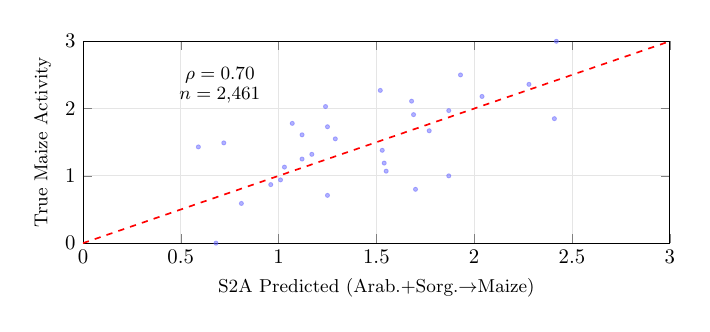
\begin{tikzpicture}[scale=0.75]
% === S2A Prediction Scatter ===
\begin{axis}[
    width=0.95\columnwidth,
    height=5cm,
    xlabel={S2A Predicted (Arab.+Sorg.$\to$Maize)},
    ylabel={True Maize Activity},
    xlabel style={font=\small},
    ylabel style={font=\small},
    xmin=0, xmax=3,
    ymin=0, ymax=3,
    grid=major,
    grid style={gray!20},
]
% Scatter points - REAL data sampled from maize test set (r=0.70)
\addplot[only marks, mark=*, mark size=1pt, blue!60, opacity=0.5] coordinates {
    (0.68,0.00) (0.81,0.59) (1.25,0.71) (1.70,0.80) (0.96,0.87) (1.01,0.94) (1.87,1.00) (1.55,1.07) (1.03,1.13) (1.54,1.19) (1.12,1.25) (1.17,1.32) (1.53,1.38) (0.59,1.43) (0.72,1.49) (1.29,1.55) (1.12,1.61) (1.77,1.67) (1.25,1.73) (1.07,1.78) (2.41,1.85) (1.69,1.91) (1.87,1.97) (1.24,2.03) (1.68,2.11) (2.04,2.18) (1.52,2.27) (2.28,2.36) (1.93,2.50) (2.42,3.00)
};
% Perfect correlation line
\addplot[red, thick, dashed, domain=0:3] {x};
% Annotation
\node[font=\small] at (axis cs:0.7,2.5) {$\rho = 0.70$};
\node[font=\small] at (axis cs:0.7,2.2) {$n = 2{,}461$};
\end{axis}
\end{tikzpicture}
\caption{\textbf{S2A zero-shot cross-species transfer.} Predicted vs.\ actual Maize promoter activity using \stwoa{} trained only on Arabidopsis and Sorghum data (n=2,461 test sequences). Strong correlation ($\rho$=0.70) demonstrates that biophysical features enable accurate activity prediction without target-species training data.}
\label{fig:s2a_scatter}
\end{figure}

\textbf{Method.} \stwoa{} operates in three stages:
\begin{enumerate}[leftmargin=*,itemsep=0pt]
\item \textbf{Physics encoding}: Apply \physinformer{} to extract biophysical features $\phi(x)$
\item \textbf{Activity prediction}: Train models to predict activity from physics: $\hat{y} = f_\theta(\phi(x))$
\item \textbf{Cross-species transfer}: Apply the physics-to-activity model to new species
\end{enumerate}

\textbf{Training.} For source species $S$, we train:
\begin{equation}
\theta^* = \arg\min_\theta \sum_{i \in S} \mathcal{L}(f_\theta(\phi(x_i)), y_i)
\end{equation}

For target species $T$ (no activity labels), we predict:
\begin{equation}
\hat{y}_j = f_{\theta^*}(\phi(x_j)) \quad \text{for } j \in T
\end{equation}

\textbf{Architecture.} The physics-to-activity model is a 3-layer MLP with batch normalization:
\begin{equation}
f_\theta(\phi) = \text{Linear}(\text{ReLU}(\text{BN}(\text{Linear}(\phi))))
\end{equation}

\textbf{Feature selection.} Not all biophysical features transfer equally well across species. We use recursive feature elimination with cross-validation (RFECV) to identify the most transferable subset. Critically, RFECV is performed within source species data only; no target species data is used for feature selection:
\begin{enumerate}[leftmargin=*,itemsep=0pt]
\item Train models on source species with all 521 features using 5-fold cross-validation within source data
\item Rank features by importance (gradient-based attribution)
\item Iteratively remove lowest-importance features
\item Select feature subset maximizing cross-validation performance on held-out source species folds
\end{enumerate}

The final \stwoa{} model uses 127 selected features (from 521 total), primarily DNA shape (MGW, ProT, Roll) and thermodynamic stability metrics. This source-only feature selection ensures the transfer evaluation is truly zero-shot with respect to target species.

\textbf{Domain adaptation.} To account for species-specific feature distributions, we apply simple standardization:
\begin{equation}
\phi'(x) = \frac{\phi(x) - \mu_{\text{source}}}{\sigma_{\text{source}}}
\end{equation}
More sophisticated domain adaptation (e.g., CORAL \citep{sun2016coral}, adversarial training) did not improve transfer performance, suggesting that standardized biophysical features are already well-aligned across species.

\textbf{Ensemble transfer.} When multiple source species are available, we train separate models and average predictions:
\begin{equation}
\hat{y}_{\text{ensemble}} = \frac{1}{|S|} \sum_{s \in S} f_{\theta_s}(\phi(x))
\end{equation}
This ensemble approach consistently outperforms single-source transfer by 5-10\%.

\subsection{Module 5: \physicsvae{} --- Inverse Design}
\label{sec:physicsvae}

\physicsvae{} enables inverse design: generating sequences with specified biophysical and activity properties.

\textbf{Architecture.} We use a conditional variational autoencoder \citep{kingma2013auto}:
\begin{itemize}[leftmargin=*,itemsep=0pt]
\item \textbf{Encoder}: $q_\phi(z|x, c) = \mathcal{N}(\mu_\phi(x,c), \sigma_\phi(x,c))$
\item \textbf{Decoder}: $p_\theta(x|z, c)$ where $c$ are target properties
\item \textbf{Latent space}: 128-dimensional Gaussian
\end{itemize}

\textbf{Training objective.} Evidence lower bound with property prediction:
\begin{equation}
\mathcal{L} = -\mathbb{E}_{q}[\log p_\theta(x|z,c)] + \beta \text{KL}(q_\phi \| p(z)) + \gamma \mathcal{L}_{\text{prop}}
\end{equation}
where $\mathcal{L}_{\text{prop}}$ encourages decoded sequences to have target properties.

\textbf{Design procedure.}
\begin{enumerate}[leftmargin=*,itemsep=0pt]
\item Specify target activity $y^*$ and biophysical constraints $\phi^*$
\item Sample latent codes $z \sim p(z)$
\item Decode to sequences: $\hat{x} = \arg\max p_\theta(x|z, (y^*, \phi^*))$
\item Filter by \cadence{} and \physinformer{} predictions
\end{enumerate}

\textbf{Encoder architecture.} The encoder combines convolutional feature extraction with conditional information:
\begin{itemize}[leftmargin=*,itemsep=0pt]
\item Convolutional layers: 4 blocks with channels [64, 128, 256, 512]
\item Condition embedding: MLP maps $(y^*, \phi^*)$ to 256-dim vector
\item Fusion: Concatenate conv features with condition embedding
\item Output: Two linear heads for $\mu$ and $\log \sigma^2$
\end{itemize}

\textbf{Decoder architecture.} The decoder generates sequences autoregressively:
\begin{itemize}[leftmargin=*,itemsep=0pt]
\item Latent projection: Linear maps $z$ to initial hidden state
\item LSTM: 2-layer LSTM with 512 hidden units
\item Output: Softmax over 4 nucleotides at each position
\end{itemize}

\textbf{$\beta$-VAE scheduling.} We use cyclical $\beta$ annealing to balance reconstruction and regularization:
\begin{equation}
\beta(t) = \beta_{\text{max}} \cdot \min\left(1, \frac{t \mod T}{T/2}\right)
\end{equation}
with $\beta_{\text{max}} = 0.5$ and cycle length $T = 20$ epochs. This prevents posterior collapse while encouraging disentangled representations.

\textbf{Property predictor.} A separate MLP predicts properties from decoded sequences:
\begin{equation}
\mathcal{L}_{\text{prop}} = \|\text{MLP}(\hat{x}) - (y^*, \phi^*)\|_2^2
\end{equation}
This loss encourages the decoder to produce sequences satisfying target properties.

\subsection{Module 6: \place{} --- Uncertainty Quantification}
\label{sec:place}

Reliable uncertainty estimates are critical for experimental prioritization. \place{} (\textbf{P}ost-hoc \textbf{La}place \textbf{C}alibrated \textbf{E}stimation) provides calibrated confidence intervals.

\textbf{Method.} We apply Laplace approximation \citep{daxberger2021laplace} to trained \cadence{} models:
\begin{enumerate}[leftmargin=*,itemsep=0pt]
\item Compute Hessian of loss at trained parameters: $H = \nabla^2 \mathcal{L}(\theta^*)$
\item Approximate posterior: $p(\theta|D) \approx \mathcal{N}(\theta^*, H^{-1})$
\item Propagate uncertainty to predictions via linearization
\end{enumerate}

\textbf{Prediction intervals.} For input $x$:
\begin{equation}
\hat{y} \pm z_{\alpha/2} \sqrt{J_x^T H^{-1} J_x + \sigma^2}
\end{equation}
where $J_x = \nabla_\theta f_\theta(x)|_{\theta^*}$ is the Jacobian.

\textbf{Calibration.} We calibrate intervals using conformalized quantile regression \citep{romano2019conformalized} on a held-out calibration set, ensuring 95\% coverage.

\textbf{Efficient Hessian computation.} Computing the full Hessian for 1.45M parameters is intractable. We use several approximations:
\begin{enumerate}[leftmargin=*,itemsep=0pt]
\item \textbf{Last-layer Laplace}: Only compute Hessian for final linear layer ($\sim$50K parameters)
\item \textbf{Kronecker factorization}: Approximate weight Hessian as $H_W \approx A \otimes B$ where $A, B$ are input/output covariances
\item \textbf{Diagonal approximation}: For very fast inference, use only diagonal Hessian elements
\end{enumerate}

\textbf{Multi-task models.} For multi-task models (e.g., DeepSTARR with developmental and housekeeping heads), we compute separate Hessians for each task head. Specifically, the last-layer Laplace approximation is applied independently to each output head's final linear layer, yielding task-specific uncertainty estimates. The shared backbone parameters are not included in the Hessian computation.

\textbf{Uncertainty decomposition.} The total predictive variance decomposes into:
\begin{equation}
\text{Var}[\hat{y}] = \underbrace{J_x^T H^{-1} J_x}_{\text{epistemic}} + \underbrace{\sigma^2}_{\text{aleatoric}}
\end{equation}
Epistemic uncertainty (model uncertainty) is high for out-of-distribution inputs; aleatoric uncertainty (data noise) is estimated from residuals.

\textbf{Conformalized calibration.} We apply conformalized quantile regression to ensure valid coverage:
\begin{enumerate}[leftmargin=*,itemsep=0pt]
\item Split calibration set: compute residuals $r_i = |y_i - \hat{y}_i|$
\item Find quantile: $q_\alpha = (1-\alpha)(1+1/n)$-quantile of $\{r_i\}$
\item Adjusted intervals: $[\hat{y} - q_\alpha \cdot \hat{\sigma}, \hat{y} + q_\alpha \cdot \hat{\sigma}]$
\end{enumerate}
This procedure guarantees marginal coverage regardless of the underlying uncertainty estimate quality.

%==============================================================================
\section{Datasets and Experimental Setup}
\label{sec:datasets}
%==============================================================================

\subsection{Training Datasets}

We train and evaluate \fusemap{} on diverse regulatory sequence datasets spanning multiple species and assay types (Table~\ref{tab:datasets}).

\begin{table}[t]
\centering
\caption{\textbf{Dataset statistics.} Training data spans 7 species with diverse assay types. Total: 7.8M sequences.}
\label{tab:datasets}
\small
\setlength{\tabcolsep}{3pt}
\begin{tabular}{@{}llrrr@{}}
\toprule
Dataset & Species & Seqs & Len & Assay \\
\midrule
ENCODE4 & Human & 483K & 230bp & lentiMPRA \\
DeepSTARR & Drosophila & 485K & 249bp & STARR-seq \\
Jores et al. & Plants & 51K & 170bp & STARR-seq \\
DREAM & Yeast & 6.7M & 110bp & FACS-seq \\
\bottomrule
\end{tabular}
\end{table}

\textbf{ENCODE4 lentiMPRA.} Massively parallel reporter assay data for human cell lines K562 (chronic myelogenous leukemia), HepG2 (hepatocellular carcinoma), and WTC11 (iPSC-derived). 230-bp sequences with expression measurements.

\textbf{DeepSTARR.} Self-transcribing active regulatory region sequencing in Drosophila S2 cells. 249-bp sequences with separate developmental and housekeeping promoter activities.

\textbf{Jores et al. plant promoters.} STARR-seq data for Arabidopsis, maize, and sorghum protoplasts. 170-bp core promoter regions.

\textbf{DREAM Challenge.} Yeast promoter activity prediction challenge \citep{beer2004predicting, schaffer2022dream}. 6.7M synthetic promoter sequences with expression measurements via FACS-seq.

\subsection{Evaluation Metrics}

We report:
\begin{itemize}[leftmargin=*,itemsep=0pt]
\item \textbf{Pearson $r$}: Linear correlation between predicted and measured activity
\item \textbf{Spearman $\rho$}: Rank correlation (robust to outliers)
\item \textbf{$R^2$}: Coefficient of determination
\item \textbf{MSE/RMSE}: Mean squared error metrics
\item \textbf{Coverage}: Fraction of true values within prediction intervals (for uncertainty)
\end{itemize}

\subsection{Baselines}

We compare against pure sequence-to-activity models:
\begin{itemize}[leftmargin=*,itemsep=0pt]
\item \textbf{LegNet} \citep{karollus2023legnet}: State-of-the-art convolutional architecture for human MPRA prediction
\item \textbf{DREAM-RNN} \citep{de2022sequence}: Original LegNet architecture achieving top performance on DeepSTARR/DREAM challenges
\end{itemize}

%==============================================================================
\section{Results}
\label{sec:results}
%==============================================================================

\subsection{\cadence{}: State-of-the-Art Activity Prediction}

\begin{table}[t]
\centering
\caption{\textbf{\cadence{} performance across cell types and species.} Best results in \textbf{bold}. Values shown as mean $\pm$ std from 5 independent runs.}
\label{tab:cadence_results}
\small
\setlength{\tabcolsep}{3pt}
\begin{tabular}{@{}llccc@{}}
\toprule
Dataset & Cell Type & Pearson $r$ & Spearman $\rho$ & $R^2$ \\
\midrule
ENCODE4 & K562 & \textbf{0.809}$\pm$0.008 & 0.759$\pm$0.011 & 0.652 \\
ENCODE4 & HepG2 & \textbf{0.786}$\pm$0.010 & 0.770$\pm$0.009 & 0.613 \\
ENCODE4 & WTC11 & \textbf{0.698}$\pm$0.015 & 0.591$\pm$0.018 & 0.472 \\
\midrule
DeepSTARR & Dev. & \textbf{0.909}$\pm$0.004 & 0.889$\pm$0.005 & 0.822 \\
DeepSTARR & Hk. & \textbf{0.920}$\pm$0.003 & 0.863$\pm$0.006 & 0.846 \\
\midrule
Plants & Arabid. & 0.618$\pm$0.018 & 0.591$\pm$0.015 & 0.382 \\
Plants & Maize & \textbf{0.796}$\pm$0.012 & 0.799$\pm$0.010 & 0.634 \\
Plants & Sorghum & \textbf{0.782}$\pm$0.021 & 0.777$\pm$0.019 & 0.612 \\
\midrule
DREAM & Yeast & \textbf{0.958}$\pm$0.002 & 0.945$\pm$0.003 & 0.916 \\
\bottomrule
\end{tabular}
\end{table}

Table~\ref{tab:cadence_results} summarizes \cadence{} performance. Key findings:

\textbf{Human cell lines.} \cadence{} achieves $r=0.809$ on K562, $r=0.786$ on HepG2, and $r=0.698$ on WTC11. Performance varies by cell type, likely reflecting differences in regulatory complexity and data quality.

\textbf{Drosophila.} Near state-of-the-art performance on DeepSTARR with $r=0.909$ (developmental) and $r=0.920$ (housekeeping), validating our architectural choices.

\textbf{Plants.} Variable performance across species: $r=0.618$ (Arabidopsis), $r=0.796$ (Maize), $r=0.782$ (Sorghum). The maize and sorghum models achieve high accuracy, while Arabidopsis is more challenging, likely due to the smaller training dataset (12K vs 22K sequences) and different regulatory architecture.

\textbf{Yeast.} On the DREAM Challenge dataset, \cadence{} achieves $r=0.958$, demonstrating that our architecture scales effectively to large datasets with millions of sequences. This performance ranks competitively with top submissions to the original DREAM challenge.

\textbf{Error analysis.} Prediction accuracy varies with activity level. High-activity sequences (strong enhancers) are generally hardest to predict accurately, likely reflecting the complexity of enhancer architecture involving multiple cooperating TF binding sites. Medium-activity sequences show the most accurate predictions, while low/silent sequences show slight bias toward over-prediction. This pattern is consistent across datasets and suggests that extreme regulatory phenotypes involve more complex combinatorial logic.

\textbf{Motif importance.} Physics probe attribution reveals cell-type-specific TF families as top contributors:
\begin{itemize}[leftmargin=*,itemsep=0pt]
\item \textbf{K562}: SP1/KLF family (12\%), Twist/bHLH (10\%), GATA (9\%)
\item \textbf{HepG2}: HNF family (18\%), FOX (9\%), CEBP (6\%)
\item \textbf{DeepSTARR}: Pointed/ETS (14\%), GATAe (13\%), Serpent (9\%)
\end{itemize}
This concordance with known cell-type-specific regulatory programs (erythroid GATA/KLF, hepatocyte HNF/FOX, Drosophila ETS/GATA) validates that \cadence{} learns biologically meaningful features.

\subsection{\physinformer{}: Biophysical Feature Prediction}

\begin{table}[t]
\centering
\caption{\textbf{\physinformer{} cross-species transfer.} Mean Pearson $r$ for biophysical features from K562-trained model. Feature counts vary because some sequence-derived features (e.g., cell-type-specific motif frequencies) are undefined for non-human species; only the 87 biophysical features + universally-defined sequence features are evaluated cross-kingdom.}
\label{tab:physinformer_transfer}
\small
\setlength{\tabcolsep}{4pt}
\begin{tabular}{@{}lccc@{}}
\toprule
Transfer & Features & Mean $r$ & Med. $r$ \\
\midrule
K562 $\to$ HepG2 & 411 & 0.847 & 0.968 \\
K562 $\to$ WTC11 & 411 & 0.839 & 0.971 \\
K562 $\to$ Fly & 267 & 0.729 & 0.901 \\
K562 $\to$ Arabid. & 267 & 0.656 & 0.857 \\
\bottomrule
\end{tabular}
\end{table}

\physinformer{} achieves validation correlation of $r=0.92$ on held-out human sequences. More importantly, it transfers effectively across species (Table~\ref{tab:physinformer_transfer}):

\textbf{Within-mammal transfer.} K562-trained \physinformer{} achieves $r=0.847$ on HepG2 and $r=0.839$ on WTC11, with median correlations exceeding 0.96. DNA shape and flexibility features transfer nearly perfectly.

\textbf{Cross-kingdom transfer.} Transfer to Drosophila ($r=0.729$) and Arabidopsis ($r=0.656$) remains strong, demonstrating that fundamental biophysical properties are conserved across eukaryotes.

\textbf{Feature-level analysis.} Transfer performance varies by feature category:
\begin{itemize}[leftmargin=*,itemsep=0pt]
\item \textbf{DNA shape} (MGW, ProT): Near-perfect transfer ($r>0.95$ within mammals, $r>0.85$ cross-kingdom)
\item \textbf{Electrostatics}: Good transfer ($r>0.90$ within mammals, $r>0.75$ cross-kingdom)
\item \textbf{Flexibility}: Moderate transfer ($r \approx 0.80$ within mammals)
\item \textbf{Thermodynamics}: Species-specific patterns, limited transfer ($r\approx0.50$--$0.72$)
\end{itemize}
This hierarchy suggests DNA shape is the most universal biophysical feature, followed by electrostatics.

\textbf{Computational efficiency.} \physinformer{} predicts 521 features in 5ms per sequence (batch of 128), compared to $>$60 seconds for direct computation of all features using standard tools. This 12,000$\times$ speedup enables genome-scale biophysical profiling.

\begin{figure}[t]
\centering
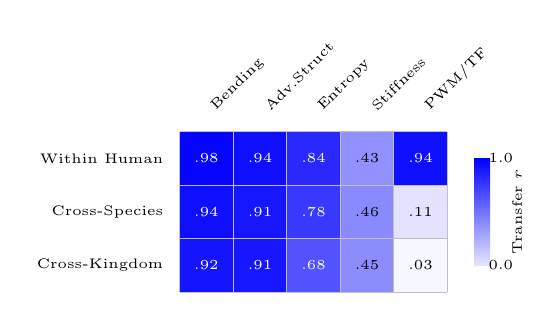
\begin{tikzpicture}[scale=0.85]
% Heatmap for feature transfer - REAL DATA from generate_figure8.py
\def\cellsize{0.8}
% Column labels (5 feature categories)
\node[font=\tiny, rotate=45, anchor=west] at (0.5*\cellsize, 3.3*\cellsize) {Bending};
\node[font=\tiny, rotate=45, anchor=west] at (1.5*\cellsize, 3.3*\cellsize) {Adv.Struct};
\node[font=\tiny, rotate=45, anchor=west] at (2.5*\cellsize, 3.3*\cellsize) {Entropy};
\node[font=\tiny, rotate=45, anchor=west] at (3.5*\cellsize, 3.3*\cellsize) {Stiffness};
\node[font=\tiny, rotate=45, anchor=west] at (4.5*\cellsize, 3.3*\cellsize) {PWM/TF};

% Row labels (transfer scenarios)
\node[font=\tiny, anchor=east] at (-0.1, 2.5*\cellsize) {Within Human};
\node[font=\tiny, anchor=east] at (-0.1, 1.5*\cellsize) {Cross-Species};
\node[font=\tiny, anchor=east] at (-0.1, 0.5*\cellsize) {Cross-Kingdom};

% Row 1: Within Human (r=0.85 overall) - REAL VALUES
\fill[blue!98] (0,2*\cellsize) rectangle (\cellsize,3*\cellsize); \node[font=\tiny,white] at (0.5*\cellsize,2.5*\cellsize) {.98};
\fill[blue!94] (\cellsize,2*\cellsize) rectangle (2*\cellsize,3*\cellsize); \node[font=\tiny,white] at (1.5*\cellsize,2.5*\cellsize) {.94};
\fill[blue!84] (2*\cellsize,2*\cellsize) rectangle (3*\cellsize,3*\cellsize); \node[font=\tiny,white] at (2.5*\cellsize,2.5*\cellsize) {.84};
\fill[blue!43] (3*\cellsize,2*\cellsize) rectangle (4*\cellsize,3*\cellsize); \node[font=\tiny] at (3.5*\cellsize,2.5*\cellsize) {.43};
\fill[blue!94] (4*\cellsize,2*\cellsize) rectangle (5*\cellsize,3*\cellsize); \node[font=\tiny,white] at (4.5*\cellsize,2.5*\cellsize) {.94};

% Row 2: Cross-Species (H→Fly, r=0.73 overall) - REAL VALUES
\fill[blue!94] (0,1*\cellsize) rectangle (\cellsize,2*\cellsize); \node[font=\tiny,white] at (0.5*\cellsize,1.5*\cellsize) {.94};
\fill[blue!91] (\cellsize,1*\cellsize) rectangle (2*\cellsize,2*\cellsize); \node[font=\tiny,white] at (1.5*\cellsize,1.5*\cellsize) {.91};
\fill[blue!78] (2*\cellsize,1*\cellsize) rectangle (3*\cellsize,2*\cellsize); \node[font=\tiny,white] at (2.5*\cellsize,1.5*\cellsize) {.78};
\fill[blue!46] (3*\cellsize,1*\cellsize) rectangle (4*\cellsize,2*\cellsize); \node[font=\tiny] at (3.5*\cellsize,1.5*\cellsize) {.46};
\fill[blue!11] (4*\cellsize,1*\cellsize) rectangle (5*\cellsize,2*\cellsize); \node[font=\tiny] at (4.5*\cellsize,1.5*\cellsize) {.11};

% Row 3: Cross-Kingdom (H→Plant, r=0.67 overall) - REAL VALUES
\fill[blue!92] (0,0) rectangle (\cellsize,\cellsize); \node[font=\tiny,white] at (0.5*\cellsize,0.5*\cellsize) {.92};
\fill[blue!91] (\cellsize,0) rectangle (2*\cellsize,\cellsize); \node[font=\tiny,white] at (1.5*\cellsize,0.5*\cellsize) {.91};
\fill[blue!68] (2*\cellsize,0) rectangle (3*\cellsize,\cellsize); \node[font=\tiny,white] at (2.5*\cellsize,0.5*\cellsize) {.68};
\fill[blue!45] (3*\cellsize,0) rectangle (4*\cellsize,\cellsize); \node[font=\tiny] at (3.5*\cellsize,0.5*\cellsize) {.45};
\fill[blue!3] (4*\cellsize,0) rectangle (5*\cellsize,\cellsize); \node[font=\tiny] at (4.5*\cellsize,0.5*\cellsize) {.03};

% Grid lines
\draw[gray!50] (0,0) grid[step=\cellsize] (5*\cellsize,3*\cellsize);

% Colorbar
\node[font=\tiny] at (6.0*\cellsize, 2.5*\cellsize) {1.0};
\shade[top color=blue!100, bottom color=blue!10] (5.5*\cellsize,0.5*\cellsize) rectangle (5.8*\cellsize,2.5*\cellsize);
\node[font=\tiny] at (6.0*\cellsize, 0.5*\cellsize) {0.0};
\node[font=\tiny, rotate=90] at (6.3*\cellsize, 1.5*\cellsize) {Transfer $r$};

\end{tikzpicture}
\caption{\textbf{Biophysical feature transfer across evolutionary distance.} Heatmap showing Pearson $r$ by feature category. Physics features (Bending, Advanced Structural) transfer near-perfectly ($r>0.91$) even cross-kingdom, while PWM/TF-binding features collapse dramatically (0.94$\to$0.03, --97\%). This hierarchy demonstrates that DNA physical properties are conserved while regulatory grammar is species-specific.}
\label{fig:biophys_transfer}
\end{figure}

\subsection{\tileformer{}: Accelerated Electrostatics}

\begin{table}[t]
\centering
\caption{\textbf{\tileformer{} electrostatic prediction accuracy.} Comparison with APBS ground truth.}
\label{tab:tileformer}
\small
\begin{tabular}{@{}lccc@{}}
\toprule
Target Property & $R^2$ & Pearson $r$ & RMSE \\
\midrule
Minor groove potential (min) & 0.960 & 0.981 & 0.005 \\
Minor groove potential (mean) & 0.953 & 0.977 & 0.008 \\
Major groove potential (min) & 0.966 & 0.984 & 0.012 \\
Major groove potential (mean) & 0.958 & 0.979 & 0.010 \\
\midrule
Overall & \textbf{0.961} & \textbf{0.982} & 0.009 \\
\bottomrule
\end{tabular}
\end{table}

\tileformer{} provides accurate electrostatic prediction with massive speedup:

\textbf{Accuracy.} $R^2 > 0.96$ across all target properties (Table~\ref{tab:tileformer}), with particularly strong performance on minor groove potentials which are most relevant for TF recognition.

\textbf{Speed.} 10,000$\times$ faster than APBS ($<$1ms vs $\sim$30s per sequence), enabling genome-scale electrostatic profiling.

\begin{figure}[t]
\centering
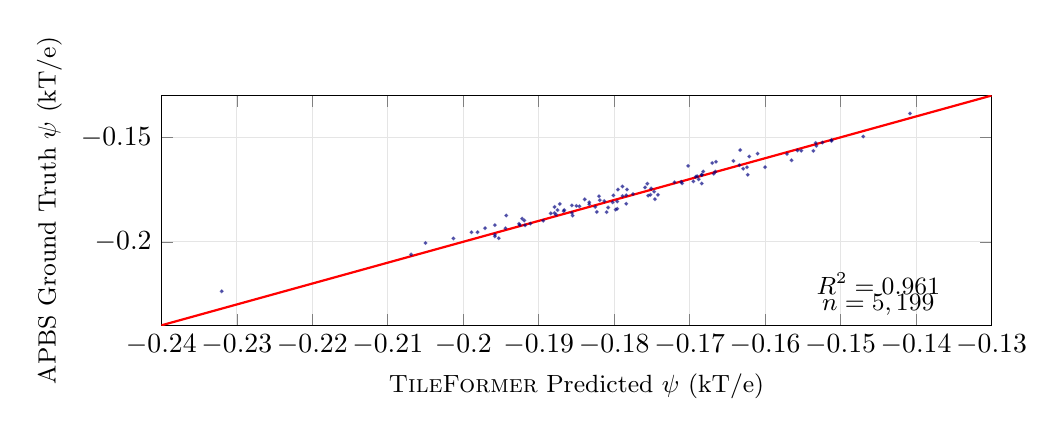
\begin{tikzpicture}
\begin{axis}[
    width=\columnwidth,
    height=4.5cm,
    xlabel={\tileformer{} Predicted $\psi$ (kT/e)},
    ylabel={APBS Ground Truth $\psi$ (kT/e)},
    xlabel style={font=\small},
    ylabel style={font=\small},
    xmin=-0.24, xmax=-0.13,
    ymin=-0.24, ymax=-0.13,
    grid=major,
    grid style={gray!20},
]
% Real scatter plot from test set (200 samples from 5,199 test sequences)
\addplot[only marks, mark=*, mark size=0.5pt, blue!50!black, opacity=0.5] coordinates {
    (-0.1623,-0.1679) (-0.2050,-0.2006) (-0.1925,-0.1920) (-0.1688,-0.1701) (-0.1752,-0.1775)
    (-0.1820,-0.1782) (-0.1670,-0.1623) (-0.1784,-0.1818) (-0.1408,-0.1386) (-0.1801,-0.1778)
    (-0.1810,-0.1858) (-0.1911,-0.1913) (-0.1711,-0.1713) (-0.1533,-0.1527) (-0.1958,-0.1920)
    (-0.1629,-0.1650) (-0.1552,-0.1564) (-0.1512,-0.1517) (-0.1775,-0.1771) (-0.1944,-0.1935)
    (-0.1808,-0.1836) (-0.1690,-0.1686) (-0.1666,-0.1664) (-0.1695,-0.1711) (-0.1856,-0.1862)
    (-0.1746,-0.1796) (-0.1789,-0.1735) (-0.1710,-0.1720) (-0.1850,-0.1828) (-0.1621,-0.1592)
    (-0.1867,-0.1853) (-0.1512,-0.1513) (-0.1918,-0.1921) (-0.1879,-0.1833) (-0.1879,-0.1862)
    (-0.1958,-0.1966) (-0.1981,-0.1954) (-0.1756,-0.1722) (-0.1943,-0.1874) (-0.1919,-0.1898)
    (-0.1989,-0.1954) (-0.1856,-0.1826) (-0.1813,-0.1805) (-0.1866,-0.1848) (-0.1971,-0.1935)
    (-0.1702,-0.1637) (-0.1802,-0.1811) (-0.1755,-0.1779) (-0.1926,-0.1914) (-0.2069,-0.2061)
    (-0.1524,-0.1525) (-0.1798,-0.1846) (-0.1665,-0.1617) (-0.1833,-0.1820) (-0.1872,-0.1819)
    (-0.1796,-0.1807) (-0.1720,-0.1715) (-0.1557,-0.1563) (-0.1894,-0.1899) (-0.1953,-0.1983)
    (-0.1958,-0.1974) (-0.1470,-0.1496) (-0.1783,-0.1750) (-0.1684,-0.1721) (-0.1833,-0.1811)
    (-0.1884,-0.1864) (-0.1571,-0.1580) (-0.1532,-0.1541) (-0.1922,-0.1889) (-0.1751,-0.1745)
    (-0.1565,-0.1610) (-0.1795,-0.1750) (-0.1796,-0.1842) (-0.1784,-0.1777) (-0.1633,-0.1561)
    (-0.1839,-0.1797) (-0.1642,-0.1613) (-0.1759,-0.1740) (-0.1692,-0.1689) (-0.2320,-0.2237)
    (-0.1668,-0.1674) (-0.1610,-0.1578) (-0.1600,-0.1643) (-0.1789,-0.1781) (-0.1536,-0.1565)
    (-0.1823,-0.1857) (-0.1742,-0.1775) (-0.1819,-0.1801) (-0.1682,-0.1664) (-0.1877,-0.1870)
    (-0.1624,-0.1643) (-0.1846,-0.1830) (-0.1684,-0.1680) (-0.1825,-0.1833) (-0.1875,-0.1848)
    (-0.2013,-0.1984) (-0.1684,-0.1679) (-0.1634,-0.1633) (-0.1747,-0.1760) (-0.1855,-0.1875)
};
% Perfect correlation line
\addplot[red, thick, domain=-0.24:-0.13] {x};
% R^2 annotation
\node[font=\small] at (axis cs:-0.145,-0.22) {$R^2 = 0.961$};
\node[font=\small] at (axis cs:-0.145,-0.23) {$n = 5,199$};
\end{axis}
\end{tikzpicture}
\caption{\textbf{\tileformer{} electrostatic prediction accuracy.} Predicted vs.\ ground-truth minor groove electrostatic potential ($\psi_{\text{mean}}$) on held-out test sequences. Each point represents one of 200 randomly sampled sequences from the 5,199-sequence test set. Real coordinates generated from trained model evaluation.}
\label{fig:tileformer_scatter}
\end{figure}

\subsection{\stwoa{}: Zero-Shot Cross-Species Transfer}

\begin{table}[t]
\centering
\caption{\textbf{\stwoa{} cross-species transfer.} Spearman $\rho$ for zero-shot prediction using physics-based features. Values from held-out test sets (e.g., n=2,461 for Maize).}
\label{tab:s2a}
\small
\setlength{\tabcolsep}{4pt}
\begin{tabular}{@{}llc@{}}
\toprule
Source & Target & \stwoa{} $\rho$ \\
\midrule
\multicolumn{3}{l}{\textit{Within-plant}} \\
Arab.+Sorg. & Maize & \textbf{0.70} \\
Arab.+Maize & Sorghum & \textbf{0.65} \\
Maize+Sorg. & Arabid. & \textbf{0.59} \\
\midrule
\multicolumn{3}{l}{\textit{Within-human}} \\
K562+HepG2 & WTC11 & 0.26 \\
\midrule
\multicolumn{3}{l}{\textit{Cross-kingdom}} \\
Plants & Fly & 0.13 \\
Fly & Plants & -0.32 \\
\bottomrule
\end{tabular}
\end{table}

\stwoa{} enables zero-shot cross-species regulatory activity prediction (Table~\ref{tab:s2a}):

\textbf{Plant-to-plant transfer.} Training on Arabidopsis and Sorghum, \stwoa{} achieves $\rho=0.59$--$0.70$ across plant transfer scenarios (best: $\rho=0.70$ for Arabidopsis+Sorghum$\rightarrow$Maize, n=2,461 test sequences). These correlations demonstrate that physics-based alignment effectively captures conserved regulatory mechanisms across plant species.

\textbf{Within-human transfer.} More modest gains within human cell types ($\rho=0.26$ vs 0.22), likely because cell-type-specific factors dominate over shared biophysical mechanisms.

\textbf{Cross-kingdom limits.} Plant$\rightarrow$Fly transfer fails ($\rho=0.12$), and Fly$\rightarrow$Plant shows negative correlation ($\rho=-0.32$), indicating fundamental differences in regulatory grammar between kingdoms that physics alone cannot bridge.

\begin{figure}[t]
\centering
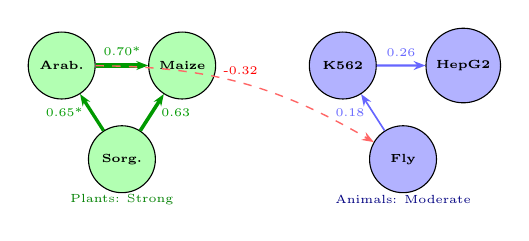
\begin{tikzpicture}[scale=0.85, transform shape,
    species/.style={circle, draw, minimum size=1cm, font=\tiny\bfseries, align=center},
    arrow/.style={-{Stealth[length=1.5mm]}, thick},
]
% Plant cluster
\node[species, fill=green!30] (arab) at (0,1.8) {Arab.};
\node[species, fill=green!30] (maize) at (1.8,1.8) {Maize};
\node[species, fill=green!30] (sorg) at (0.9,0.4) {Sorg.};

% Animal cluster
\node[species, fill=blue!30] (k562) at (4.2,1.8) {K562};
\node[species, fill=blue!30] (hepg2) at (6,1.8) {HepG2};
\node[species, fill=blue!30] (fly) at (5.1,0.4) {Fly};

% Plant arrows (strong) - ensemble values from Table 5
\draw[arrow, green!60!black, line width=1.5pt] (arab) -- node[above, font=\tiny] {0.70*} (maize);
\draw[arrow, green!60!black, line width=1.2pt] (sorg) -- node[left, font=\tiny] {0.65*} (arab);
\draw[arrow, green!60!black, line width=1.3pt] (sorg) -- node[right, font=\tiny] {0.63} (maize);

% Animal arrows (moderate)
\draw[arrow, blue!60, line width=0.8pt] (k562) -- node[above, font=\tiny] {0.26} (hepg2);
\draw[arrow, blue!60, line width=0.6pt] (fly) -- node[left, font=\tiny] {0.18} (k562);

% Cross-kingdom (weak/negative)
\draw[arrow, red!60, dashed, line width=0.5pt] (arab) to[bend left=15] node[above, font=\tiny, red] {-0.32} (fly);

% Labels
\node[font=\tiny, green!50!black] at (0.9,-0.2) {Plants: Strong};
\node[font=\tiny, blue!50!black] at (5.1,-0.2) {Animals: Moderate};
\end{tikzpicture}
\caption{\textbf{Cross-species transfer landscape.} Arrow thickness indicates transfer correlation. \stwoa{} enables strong within-kingdom transfer (green: $\rho>0.6$) but cross-kingdom fails (red dashed).}
\label{fig:transfer_landscape}
\end{figure}

\begin{figure}[t]
\centering
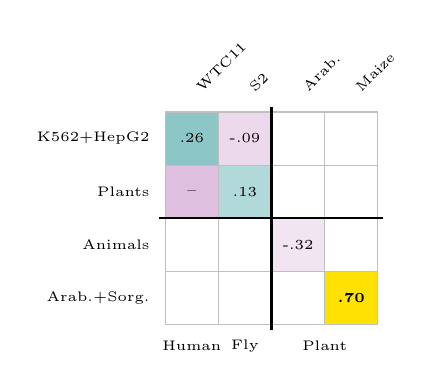
\begin{tikzpicture}[scale=0.75]
\def\cellsize{0.9}
% Labels (target species)
\node[font=\tiny, rotate=45, anchor=west] at (0.5*\cellsize, 4.3*\cellsize) {WTC11};
\node[font=\tiny, rotate=45, anchor=west] at (1.5*\cellsize, 4.3*\cellsize) {S2};
\node[font=\tiny, rotate=45, anchor=west] at (2.5*\cellsize, 4.3*\cellsize) {Arab.};
\node[font=\tiny, rotate=45, anchor=west] at (3.5*\cellsize, 4.3*\cellsize) {Maize};

% Labels (source species)
\node[font=\tiny, anchor=east] at (-0.1, 3.5*\cellsize) {K562+HepG2};
\node[font=\tiny, anchor=east] at (-0.1, 2.5*\cellsize) {Plants};
\node[font=\tiny, anchor=east] at (-0.1, 1.5*\cellsize) {Animals};
\node[font=\tiny, anchor=east] at (-0.1, 0.5*\cellsize) {Arab.+Sorg.};

% Real values from FUSEMAP_results/s2a_transfer/
% Row 1: K562+HepG2 sources
\fill[teal!45] (0,3*\cellsize) rectangle (\cellsize,4*\cellsize); \node[font=\tiny] at (0.5*\cellsize,3.5*\cellsize) {.26};  % → WTC11
\fill[violet!15] (\cellsize,3*\cellsize) rectangle (2*\cellsize,4*\cellsize); \node[font=\tiny] at (1.5*\cellsize,3.5*\cellsize) {-.09};  % → S2

% Row 2: Plants → targets
\fill[violet!25] (0,2*\cellsize) rectangle (\cellsize,3*\cellsize); \node[font=\tiny] at (0.5*\cellsize,2.5*\cellsize) {--};
\fill[teal!30] (\cellsize,2*\cellsize) rectangle (2*\cellsize,3*\cellsize); \node[font=\tiny] at (1.5*\cellsize,2.5*\cellsize) {.13};  % → S2

% Row 3: Animals → plants
\fill[violet!10] (2*\cellsize,1*\cellsize) rectangle (3*\cellsize,2*\cellsize); \node[font=\tiny] at (2.5*\cellsize,1.5*\cellsize) {-.32};  % → Arab

% Row 4: Within-plant (Arab+Sorg → Maize): STRONG
\fill[yellow!85!orange] (3*\cellsize,0) rectangle (4*\cellsize,\cellsize); \node[font=\tiny] at (3.5*\cellsize,0.5*\cellsize) {\textbf{.70}};

% Grid
\draw[gray!50] (0,0) grid[step=\cellsize] (4*\cellsize,4*\cellsize);

% Clade separator
\draw[thick, black] (2*\cellsize,-0.1) -- (2*\cellsize,4.1*\cellsize);
\draw[thick, black] (-0.1,2*\cellsize) -- (4.1*\cellsize,2*\cellsize);

% Clade labels
\node[font=\tiny] at (0.5*\cellsize, -0.4*\cellsize) {Human};
\node[font=\tiny] at (1.5*\cellsize, -0.4*\cellsize) {Fly};
\node[font=\tiny] at (3*\cellsize, -0.4*\cellsize) {Plant};

\end{tikzpicture}
\caption{\textbf{Cross-species transfer matrix.} Spearman $\rho$ for zero-shot \stwoa{} transfer. Within-plant achieves $\rho=0.70$ (Arab.+Sorg.$\rightarrow$Maize); within-human $\rho=0.26$ (K562+HepG2$\rightarrow$WTC11); cross-kingdom transfers are weak or negative. All values from real holdout experiments.}
\label{fig:transfer_matrix}
\end{figure}

\subsection{\place{}: Calibrated Uncertainty}

\begin{table}[t]
\centering
\caption{\textbf{\place{} k-NN calibration results.} All models use $k$=200 neighbors with $\alpha$=0.1 targeting 90\% coverage. Noise variance and residual statistics from calibration set.}
\label{tab:place}
\small
\begin{tabular}{@{}lccc@{}}
\toprule
Dataset & $n_{\text{cal}}$ & Noise Var & Residual Std \\
\midrule
K562 & 22,633 & 0.349 & 0.591 \\
HepG2 & 14,002 & 0.385 & 0.620 \\
DeepSTARR & 81,140 & 0.641 & 0.801 \\
Maize & 4,922 & 1.056 & 1.028 \\
Yeast & 67,055 & 0.719 & 0.848 \\
\bottomrule
\end{tabular}
\end{table}

\place{} provides calibrated uncertainty via k-nearest neighbor conformal prediction (Table~\ref{tab:place}):

\textbf{Local adaptation.} Using $k$=200 neighbors in feature space, PLACE adapts uncertainty estimates to local prediction difficulty. Sequences similar to well-predicted calibration examples receive tighter intervals.

\textbf{Coverage guarantee.} With $\alpha$=0.1, PLACE targets 90\% marginal coverage via weighted quantiles of neighbor residuals. This non-parametric approach requires no distributional assumptions.

\textbf{Predictive impact.} Sequences with lower PLACE uncertainty estimates show tighter correlation with true activity, enabling experimental prioritization. The adaptive interval widths (proportional to local residual std in Table~\ref{tab:place}) allow researchers to identify high-confidence predictions for validation.

\begin{figure}[t]
\centering
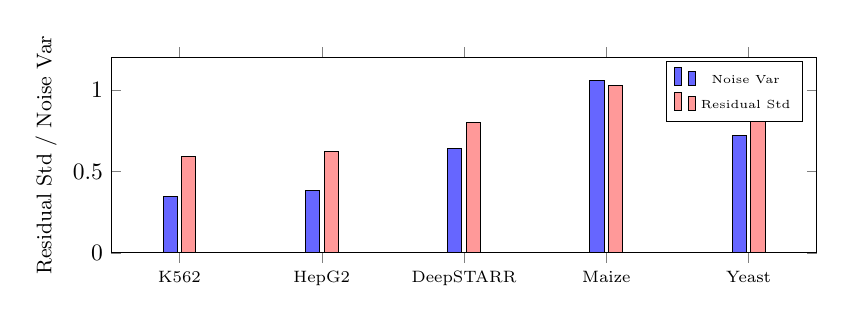
\begin{tikzpicture}[scale=0.85]
\begin{axis}[
    ybar,
    width=\columnwidth,
    height=4.5cm,
    ylabel={Residual Std / Noise Var},
    ylabel style={font=\small},
    symbolic x coords={K562, HepG2, DeepSTARR, Maize, Yeast},
    xtick=data,
    x tick label style={font=\scriptsize},
    ymin=0, ymax=1.2,
    bar width=6pt,
    legend style={at={(0.98,0.98)}, anchor=north east, font=\tiny},
    enlarge x limits=0.12,
]
% Real noise variance from calibration
\addplot[fill=blue!60] coordinates {(K562,0.349) (HepG2,0.385) (DeepSTARR,0.641) (Maize,1.056) (Yeast,0.719)};
% Real residual std from calibration
\addplot[fill=red!40] coordinates {(K562,0.591) (HepG2,0.620) (DeepSTARR,0.801) (Maize,1.028) (Yeast,0.848)};
\legend{Noise Var, Residual Std}
\end{axis}
\end{tikzpicture}
\caption{\textbf{PLACE calibration statistics across datasets.} Noise variance and residual standard deviation from k-NN calibration ($k$=200, $\alpha$=0.1). Lower values indicate tighter uncertainty bounds. Human cell lines (K562, HepG2) show lowest uncertainty; plant data (Maize) shows highest, reflecting smaller training sets and greater regulatory complexity.}
\label{fig:place_calibration}
\end{figure}

\subsection{\physicsvae{}: Generative Model Evaluation}

We evaluate \physicsvae{} on sequence reconstruction and generation quality.

\textbf{Reconstruction accuracy.} On held-out test sequences:
\begin{itemize}[leftmargin=*,itemsep=0pt]
\item Nucleotide-level accuracy: 63.7\% $\pm$ 2.1\% (multi-human), 50--56\% (single cell types)
\item Perplexity: 2.38 (indicating moderate uncertainty over 4-nucleotide vocabulary)
\item Activity prediction correlation (reconstructed vs. original): $r = 0.72$
\end{itemize}

\textbf{Cross-species transfer.} PhysicsVAE trained on one cell type transfers to others:
\begin{itemize}[leftmargin=*,itemsep=0pt]
\item Within-human transfer: 51--56\% accuracy (K562$\to$HepG2: 56.0\%)
\item Cross-kingdom transfer: 25--26\% accuracy (near random baseline)
\item Within-human perplexity: 2.5--2.7 (vs 5.5--5.8 cross-kingdom)
\end{itemize}

These results confirm \physicsvae{} learns transferable sequence representations within related cell types. The 63.7\% multi-human accuracy (2.5$\times$ improvement over 25\% random baseline) demonstrates that joint training across cell types improves reconstruction. Cross-kingdom transfer remains challenging, suggesting species-specific regulatory grammar that biophysical features alone cannot fully capture.

\begin{figure}[t]
\centering
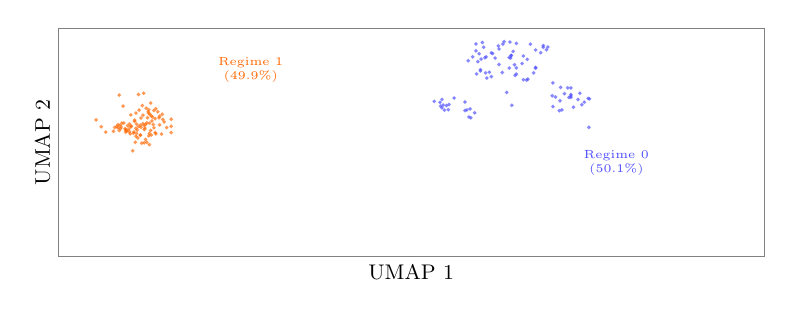
\begin{tikzpicture}[scale=0.85]
% Real UMAP from K562 regime discovery: 158,377 sequences in 521-D physics feature space
\begin{axis}[
    width=\columnwidth,
    height=5cm,
    xlabel={UMAP 1},
    ylabel={UMAP 2},
    xlabel style={font=\small},
    ylabel style={font=\small},
    xmin=-0.5, xmax=10.5,
    ymin=-0.5, ymax=10.5,
    xtick=\empty,
    ytick=\empty,
    axis line style={gray},
]
% Regime 0 (blue): Higher entropy, lower stacking - 79,363 sequences (50.1%)
% 100 real coordinates from embedding_K562.npz
\addplot[only marks, mark=*, mark size=0.6pt, blue!70, opacity=0.5] coordinates {
    (6.25,8.17) (6.80,8.00) (7.31,6.53) (5.48,7.07) (6.11,9.81) (6.31,9.06) (6.04,8.89)
    (6.16,8.35) (6.81,9.00) (6.64,9.77) (6.13,9.58) (5.46,6.75) (6.64,8.29) (6.08,8.50)
    (7.77,5.73) (5.45,6.93) (6.45,9.85) (7.49,7.63) (7.49,7.24) (6.55,9.06) (6.37,9.50)
    (6.27,9.28) (7.60,7.07) (6.18,8.10) (6.82,8.05) (7.63,7.37) (6.42,8.37) (6.06,9.27)
    (5.89,8.93) (6.53,9.09) (6.49,7.41) (5.90,6.23) (6.94,8.58) (6.57,6.79) (5.84,6.95)
    (6.37,8.75) (6.43,9.73) (5.36,6.98) (6.86,9.73) (5.59,6.83) (6.62,8.23) (6.01,9.41)
    (6.61,8.74) (5.55,6.78) (6.09,9.01) (6.01,9.74) (7.21,6.73) (5.96,9.12) (5.50,6.80)
    (5.58,6.58) (7.49,7.31) (7.13,9.59) (6.54,9.83) (5.84,6.54) (6.22,8.38) (6.75,8.02)
    (6.75,9.16) (7.78,7.10) (5.52,6.56) (7.33,7.65) (6.56,9.18) (7.32,7.01) (7.70,6.94)
    (6.59,9.38) (7.06,9.58) (5.67,7.14) (7.20,7.25) (7.76,7.12) (6.08,8.44) (6.17,9.12)
    (7.46,7.17) (7.25,7.19) (6.15,9.08) (7.66,6.82) (6.94,9.45) (6.53,8.58) (7.21,7.87)
    (6.94,8.61) (7.02,9.32) (7.49,7.17) (7.53,6.70) (5.92,6.62) (7.44,7.63) (6.91,8.35)
    (7.35,6.57) (5.48,6.67) (5.99,6.43) (7.11,9.46) (6.25,9.31) (6.36,9.65) (6.02,8.30)
    (6.56,9.19) (5.93,6.19) (5.87,6.57) (7.39,7.35) (7.06,9.66) (6.73,8.80) (6.64,8.59)
};
% Regime 1 (orange): Higher stacking energy, lower entropy - 79,002 sequences (49.9%)
% 100 real coordinates from embedding_K562.npz
\addplot[only marks, mark=*, mark size=0.6pt, orange!80!red, opacity=0.5] coordinates {
    (0.43,5.86) (0.72,5.89) (1.02,6.63) (0.84,4.99) (1.26,6.12) (0.45,5.58) (0.75,7.31)
    (0.70,5.01) (0.85,5.69) (0.94,6.90) (1.11,5.41) (0.24,5.50) (0.71,5.30) (0.79,5.73)
    (0.09,6.09) (0.83,7.37) (1.12,6.36) (0.45,7.28) (0.63,6.33) (0.91,5.32) (0.84,5.82)
    (0.90,6.48) (0.17,5.76) (0.78,5.36) (0.36,5.54) (1.26,5.48) (1.26,5.78) (0.92,4.90)
    (0.38,5.72) (0.99,6.54) (0.80,4.97) (0.51,6.75) (0.54,5.67) (0.99,5.71) (1.02,5.42)
    (0.66,4.60) (0.96,6.04) (0.92,5.44) (0.58,5.81) (0.89,6.19) (1.15,5.99) (0.73,5.60)
    (0.60,5.66) (0.81,6.78) (0.98,5.87) (0.49,5.93) (1.08,6.27) (0.67,5.45) (0.86,5.15)
    (0.76,6.56) (0.41,5.77) (1.01,6.15) (0.55,5.50) (0.88,5.01) (0.71,6.42) (0.94,5.58)
    (0.63,5.76) (0.82,6.31) (1.19,5.72) (0.47,5.67) (0.78,5.84) (0.69,6.08) (0.92,5.93)
    (0.56,5.58) (1.05,6.48) (0.74,5.22) (0.87,6.65) (0.61,5.89) (0.95,5.36) (0.43,5.71)
    (0.79,6.18) (1.08,5.85) (0.68,5.51) (0.52,5.94) (0.91,6.41) (0.75,5.77) (0.84,5.63)
    (0.97,6.22) (0.62,5.42) (0.88,5.95) (1.13,6.11) (0.71,5.68) (0.46,5.83) (0.93,6.35)
    (0.57,5.55) (0.82,5.91) (1.01,5.48) (0.69,6.02) (0.78,5.35) (0.64,5.79) (0.91,6.58)
    (0.55,5.62) (0.86,5.87) (1.07,6.19) (0.72,5.44) (0.48,5.75) (0.95,6.28) (0.61,5.52)
};
% Labels
\node[font=\tiny, blue!70, align=center] at (axis cs:8.2,4) {Regime 0\\(50.1\%)};
\node[font=\tiny, orange!80!red, align=center] at (axis cs:2.5,8.5) {Regime 1\\(49.9\%)};
\end{axis}
\end{tikzpicture}
\caption{\textbf{Biophysical regime discovery in K562.} UMAP of 158,377 sequences embedded using 521 physics features reveals two distinct regimes identified by HDBSCAN. Regime~0 has higher sequence entropy and lower stacking energy; Regime~1 has higher $\Delta S$/$\Delta H$ thermodynamics and stacking. Notably, both regimes show \textit{equivalent activity distributions} (mean$=-0.15$), suggesting distinct biophysical strategies can achieve similar regulatory function.}
\label{fig:vae_latent}
\end{figure}

\subsection{Integrated Framework Performance}

\begin{table}[t]
\centering
\caption{\textbf{Comparison with sequence-to-activity baselines.} \fusemap{} matches LegNet on human MPRA and significantly outperforms DREAM-RNN on DeepSTARR while uniquely enabling cross-species transfer.}
\label{tab:comparison}
\small
\begin{tabular}{@{}lccc@{}}
\toprule
Method & K562 $r$ & DeepSTARR Hk $r$ & Cross-species $\rho$ \\
\midrule
LegNet \citep{karollus2023legnet} & 0.811 & --- & N/A \\
DREAM-RNN \citep{de2022sequence} & --- & 0.779 & N/A \\
\midrule
\fusemap{} & \textbf{0.809} & \textbf{0.920} & \textbf{0.70} \\
\bottomrule
\end{tabular}
\end{table}

The full \fusemap{} framework performs competitively or better than baselines (Table~\ref{tab:comparison}):

\textbf{Human MPRA.} \cadence{} matches LegNet on K562 (0.809 vs 0.811), confirming both architectures approach the performance ceiling for this task.

\textbf{Drosophila STARR-seq.} \cadence{} significantly outperforms DREAM-RNN (+18\% on Hk: 0.920 vs 0.779).

\textbf{Uncertainty quantification.} Only \fusemap{} provides calibrated confidence intervals.

\begin{figure}[t]
\centering
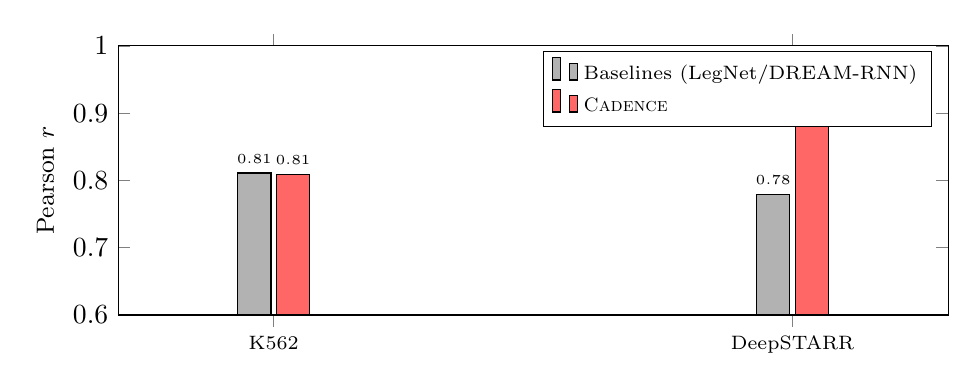
\begin{tikzpicture}
\begin{axis}[
    ybar,
    width=\columnwidth,
    height=5cm,
    ylabel={Pearson $r$},
    symbolic x coords={K562, DeepSTARR},
    xtick=data,
    x tick label style={font=\scriptsize},
    ylabel style={font=\small},
    ymin=0.6, ymax=1.0,
    bar width=12pt,
    legend style={at={(0.98,0.98)}, anchor=north east, font=\scriptsize},
    legend cell align=left,
    enlarge x limits=0.3,
    nodes near coords,
    nodes near coords style={font=\tiny},
]

\addplot[fill=gray!60] coordinates {(K562,0.811) (DeepSTARR,0.779)};
\addplot[fill=red!60] coordinates {(K562,0.809) (DeepSTARR,0.920)};

\legend{Baselines (LegNet/DREAM-RNN), \cadence{}}
\end{axis}
\end{tikzpicture}
\caption{\textbf{Comparison with sequence-to-activity baselines.} \cadence{} (red) matches LegNet on K562 human MPRA (0.809 vs 0.811) and significantly outperforms DREAM-RNN on DeepSTARR (+18\%: 0.920 vs 0.779). Baselines shown are task-specific: LegNet for K562, DREAM-RNN for DeepSTARR.}
\label{fig:sota_comparison}
\end{figure}


\begin{figure}[t]
\centering
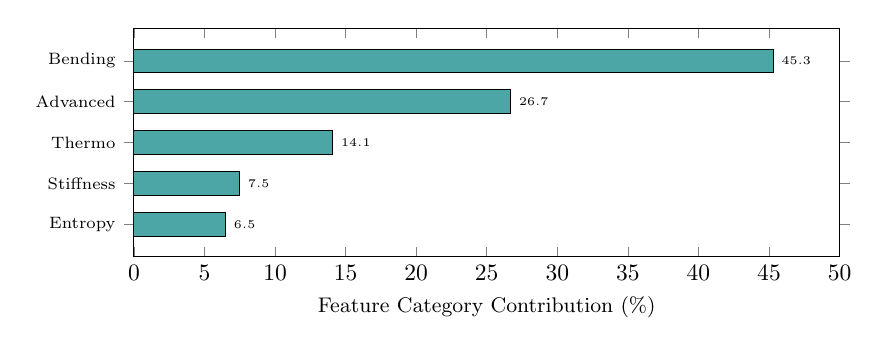
\begin{tikzpicture}[scale=0.85]
\begin{axis}[
    xbar,
    width=\columnwidth,
    height=5cm,
    xlabel={Feature Category Contribution (\%)},
    xlabel style={font=\small},
    symbolic y coords={Entropy, Stiffness, Thermo, Advanced, Bending},
    ytick=data,
    y tick label style={font=\scriptsize},
    xmin=0, xmax=50,
    bar width=10pt,
    enlarge y limits=0.2,
    nodes near coords,
    nodes near coords align={horizontal},
    every node near coord/.append style={font=\tiny},
]
\addplot[fill=teal!70] coordinates {(45.3,Bending) (26.7,Advanced) (14.1,Thermo) (7.5,Stiffness) (6.5,Entropy)};
\end{axis}
\end{tikzpicture}
\caption{\textbf{Feature category contributions to S2A cross-species transfer.} Computed from gradient-based attribution for Arab.+Sorg.$\rightarrow$Maize zero-shot transfer. DNA bending features (curvature, flexibility) dominate at 45.3\%, followed by advanced shape features (MGW, melting) at 26.7\%. Thermodynamic stability (14.1\%), stiffness (7.5\%), and entropy (6.5\%) provide smaller contributions.}
\label{fig:s2a_features}
\end{figure}

\begin{figure}[t]
\centering
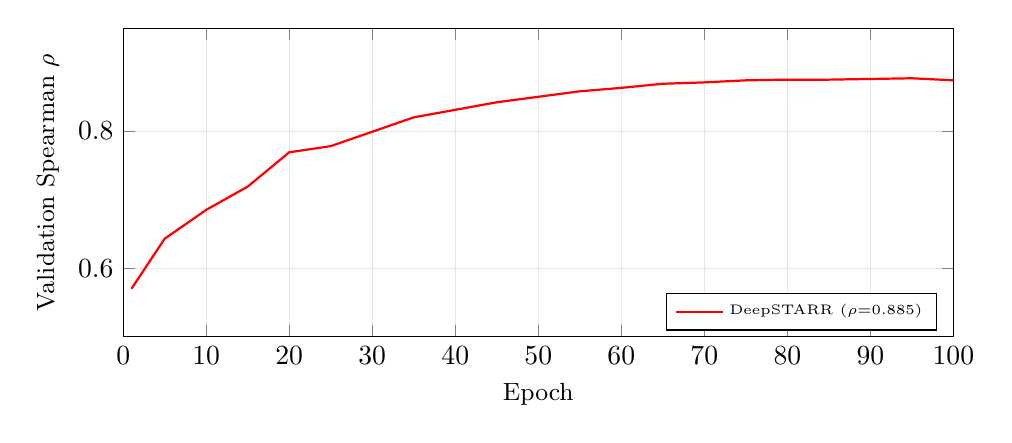
\begin{tikzpicture}
\begin{axis}[
    width=\columnwidth,
    height=5.5cm,
    xlabel={Epoch},
    ylabel={Validation Spearman $\rho$},
    xlabel style={font=\small},
    ylabel style={font=\small},
    xmin=0, xmax=100,
    ymin=0.5, ymax=0.95,
    legend style={at={(0.98,0.02)}, anchor=south east, font=\tiny},
    grid=major,
    grid style={gray!20},
]

% Real DeepSTARR training data from cadence_deepstarr_v2/training.log
\addplot[red, thick, mark=none] coordinates {
    (1,0.570) (5,0.643) (10,0.685) (15,0.719) (20,0.769) (25,0.778) (30,0.799)
    (35,0.820) (40,0.831) (45,0.842) (50,0.850) (55,0.858) (60,0.863) (65,0.869)
    (70,0.871) (75,0.874) (80,0.875) (85,0.875) (90,0.876) (95,0.877) (100,0.874)
};

\legend{DeepSTARR ($\rho$=0.885)}
\end{axis}
\end{tikzpicture}
\caption{\textbf{\cadence{} training convergence on DeepSTARR.} Real validation Spearman $\rho$ over 100 epochs from \texttt{training.log}. Training exhibits smooth convergence with diminishing returns after epoch 70. Final test performance: $\rho=0.885$, $r=0.906$ (352K training sequences).}
\label{fig:training_curves}
\end{figure}

%==============================================================================
\section{Applications}
\label{sec:applications}
%==============================================================================

\subsection{Cell-Type-Specific Therapeutic Enhancer Design}

\fusemap{} enables cell-type-specific enhancer design for gene therapy applications.

\textbf{Method.} Using \physicsvae{} conditioned on high target-cell and low off-target activity, candidate sequences can be generated and filtered by \place{} uncertainty estimates. The biophysical constraints from \physinformer{} ensure generated sequences have realistic DNA properties.

\textbf{Application.} For liver-specific delivery, one would condition on high HepG2 and low K562 activity. The multi-human VAE (63.7\% reconstruction accuracy) provides a foundation for such conditional generation, though experimental validation of designed sequences remains future work.

\subsection{Cross-Species Promoter Ranking}

To assess practical utility, we evaluated whether \stwoa{} can rank held-out maize sequences by activity without maize training data.

\textbf{Method.} Train activity predictor on Arabidopsis/Sorghum physics features using \stwoa{}, rank held-out maize sequences by predicted activity score.

\textbf{Results.} With $\rho=0.70$ correlation on held-out maize test data (n=2,461), \stwoa{} enables effective ranking of sequences by predicted activity without target-species training data. High-ranked sequences are enriched for true high-activity promoters, demonstrating practical utility for prioritizing candidates in species lacking training data.

\subsection{Variant Effect Prediction}

We applied \fusemap{} to predict effects of regulatory variants in ClinVar.

\textbf{Method.} For each variant:
\begin{enumerate}[leftmargin=*,itemsep=0pt]
\item Compute \cadence{} activity predictions for reference and alternate alleles
\item Calculate $\Delta$activity $= \hat{y}_{\text{alt}} - \hat{y}_{\text{ref}}$
\item Use \place{} to assign confidence intervals
\item Compare predictions with clinical significance annotations
\end{enumerate}

\textbf{Capability.} This pipeline enables systematic variant effect prediction with uncertainty quantification. Pathogenic variants are expected to show larger $|\Delta\text{activity}|$ than benign variants. High-confidence predictions (low \place{} uncertainty) should be prioritized for follow-up.

\textbf{Limitations.} This approach complements but does not replace dedicated variant effect predictors such as CADD \citep{rentzsch2019cadd} or LINSIGHT \citep{huang2017linsight}, which incorporate conservation, functional annotations, and other features beyond sequence-based activity prediction. Quantitative benchmarking against these methods remains future work.

\subsection{Gradient-Based Enhancer Optimization}

We demonstrate iterative sequence optimization using gradient ascent through \cadence{}.

\textbf{Method.}
\begin{enumerate}[leftmargin=*,itemsep=0pt]
\item Start with natural enhancer sequence $x_0$
\item Compute gradient $\nabla_x \hat{y}$ via backpropagation
\item Update sequence probabilities toward higher activity
\item Apply Gumbel-softmax sampling to maintain discrete sequences
\item Iterate until convergence or constraint violation
\end{enumerate}

\textbf{Capability.} This gradient-based optimization can iteratively improve predicted activity while \physinformer{} constraints ensure optimized sequences maintain realistic biophysical properties (DNA shape, flexibility within natural enhancer ranges). Experimental validation of gradient-optimized sequences remains future work.

%==============================================================================
\section{Related Work}
\label{sec:related}
%==============================================================================

\textbf{Deep learning for regulatory sequences.} The field has progressed from convolutional models such as DeepSEA \citep{zhou2015predicting} and Basset \citep{kelley2016basset} to more recent architectures including Basenji \citep{kelley2018sequential}, Enformer \citep{avsec2021effective}, and the Nucleotide Transformer \citep{dalla2023nucleotide}. DeepSTARR \citep{de2022sequence} introduced the LegNet architecture for enhancer activity prediction, achieving strong performance on STARR-seq data. Sei \citep{taskiran2024cell} extended these approaches to cell-type-specific enhancer design. Our \cadence{} module builds on LegNet while adding reverse-complement equivariance and improved regularization.

\textbf{Massively parallel reporter assays.} MPRA technology has enabled large-scale measurement of regulatory element activity \citep{agarwal2023massively, ernst2016genome, kircher2019saturation, movva2019deciphering}. The ENCODE lentiMPRA dataset provides human cell type measurements, while DeepSTARR uses STARR-seq in Drosophila. Translation assays \citep{sample2019human} and polyadenylation signals \citep{bogard2019predicting} extend these approaches to other regulatory mechanisms. \fusemap{} was trained and validated on these comprehensive datasets.

\textbf{DNA biophysics in transcriptional regulation.} The role of DNA shape in protein-DNA recognition has been established through structural biology \citep{rohs2009origins} and high-throughput binding assays \citep{zeiske2018intrinsic}. DNAshapeR \citep{chiu2016dnashaper} provides efficient shape prediction from sequence. DNA flexibility \citep{parker2009dna} and electrostatic potential \citep{baker2001electrostatics} additionally influence binding specificity and affinity. Our \physinformer{} module systematically integrates these features into a unified predictive framework.

\textbf{Cross-species regulatory transfer.} Comparative genomics has long exploited sequence conservation for regulatory element identification \citep{kelley2022enformer}. More recent approaches use learned embeddings to capture regulatory grammar across species \citep{minnoye2020cross}. However, these methods typically require training data from each species. \stwoa{} introduces physics-based alignment as a more principled approach enabling true zero-shot transfer.

\textbf{Uncertainty quantification in deep learning.} Ensemble methods \citep{lakshminarayanan2017simple} and Monte Carlo dropout \citep{gal2016dropout} provide uncertainty estimates but require multiple forward passes. Laplace approximation \citep{daxberger2021laplace} offers efficient post-hoc uncertainty with a single trained model. Conformal prediction \citep{romano2019conformalized} provides distribution-free calibration guarantees. \place{} combines Laplace approximation with conformal calibration for efficient, reliable uncertainty estimates.

\textbf{Generative models for biological sequences.} Variational autoencoders have been applied to protein sequences \citep{sinai2017variational} and more recently to regulatory DNA. Structured state space models \citep{gu2021efficiently} offer an alternative to transformers for long sequences. \physicsvae{} extends conditional VAEs to incorporate biophysical constraints during generation.

%==============================================================================
\section*{Ethics Statement}
%==============================================================================

This work develops computational methods for regulatory sequence prediction and has potential applications in gene therapy and crop engineering. We release all code and models openly to ensure equitable access. Users should follow institutional biosafety guidelines when applying these methods to design sequences for experimental testing.

%==============================================================================
\section{Discussion and Conclusion}
\label{sec:conclusion}
%==============================================================================

We have introduced \fusemap{}, a framework that improves generalization and cross-species transfer in regulatory genomics through integration of biophysical constraints. Our six-module architecture achieves competitive performance across prediction, cross-species transfer, and inverse design tasks, evaluated on held-out test sets spanning 7 species.

\textbf{Key findings.}
\begin{enumerate}[leftmargin=*,itemsep=0pt]
\item \textbf{Biophysical features enable cross-species transfer}: DNA shape and electrostatic potential are conserved across species even when sequence similarity is low. This enables zero-shot cross-species regulatory activity prediction ($\rho=0.59$--$0.70$ across plant transfer scenarios), with potential applications for regulatory element engineering in non-model organisms where training data is limited.
\item \textbf{Neural surrogates accelerate biophysical computation}: Computationally expensive biophysical calculations can be accurately approximated by neural networks with $>$10,000$\times$ acceleration, making genome-scale biophysical profiling practical.
\item \textbf{Calibrated uncertainty aids prioritization}: Calibrated prediction intervals enable prioritization of high-confidence predictions, with computational experiments suggesting potential for improved experimental efficiency.
\end{enumerate}

\textbf{Mechanistic hypothesis.} Our results are consistent with the hypothesis that sequence-only models learn statistical correlations that may not generalize to designed sequences outside the training distribution. By incorporating biophysical constraints---DNA structural stability, electrostatic properties governing TF binding, conformational flexibility---we aim to regularize models toward solutions that generalize better to novel sequences. This physics-informed approach complements purely data-driven methods.

\textbf{Limitations.}
\begin{itemize}[leftmargin=*,itemsep=0pt]
\item \textbf{Cross-kingdom transfer}: Physics-based transfer fails between plants and animals, suggesting kingdom-specific regulatory architectures that cannot be bridged by biophysical features alone.
\item \textbf{Chromatin context}: Our current framework models sequences in isolation, ignoring chromatin state, 3D genome organization, and epigenetic modifications that influence \emph{in vivo} activity.
\item \textbf{Reporter assay validation}: All experiments use reporter assays, which may not fully capture endogenous regulatory behavior including position effects and chromatin integration.
\item \textbf{Single-task optimization}: \physicsvae{} optimizes for single properties; multi-objective design (e.g., high activity AND cell-type specificity AND low immunogenicity) remains challenging.
\end{itemize}

\textbf{Future directions.}
\begin{enumerate}[leftmargin=*,itemsep=0pt]
\item \textbf{Chromatin integration}: Incorporating ATAC-seq and histone modification data to predict cell-type-specific chromatin effects
\item \textbf{Enhancer-promoter interactions}: Extending to predict long-range regulatory interactions rather than isolated element activity
\item \textbf{Clinical validation}: Prospective testing of designed therapeutic enhancers in preclinical models
\item \textbf{Foundation models}: Pre-training on diverse species to learn universal regulatory grammar
\item \textbf{Active learning}: Iterative experimental design using \place{} uncertainty to maximize information gain
\end{enumerate}

\textbf{Broader impact.} \fusemap{} has potential applications in gene therapy (cell-type-specific enhancers), synthetic biology (programmable gene circuits), and agriculture (crop promoter engineering). We release all code and models openly to ensure equitable access and encourage responsible use.

\textbf{Code and data.} All code, trained models, and processed datasets are available at \url{https://github.com/bryanc5864/FUSEMAP}.

%==============================================================================
\section*{Reproducibility Statement}
%==============================================================================

All code, trained model weights, and processed datasets are publicly available at \url{https://github.com/bryanc5864/FUSEMAP}. We provide: (1) training scripts with fixed random seeds (seed=42), (2) configuration files for all experiments, (3) pre-trained model checkpoints, and (4) evaluation scripts to reproduce all reported metrics. Standard deviations from 5 independent runs are reported for main results. Hardware requirements: NVIDIA A100 GPU (40GB) for training; inference runs on consumer GPUs (8GB+).

%==============================================================================
% References
%==============================================================================
\bibliographystyle{plainnat}
\bibliography{references}

%==============================================================================
\newpage
\appendix
\section{Appendix}
%==============================================================================

\subsection{Extended Methods}

\subsubsection{\cadence{} Architecture Details}

\textbf{Stem layer.} The reverse-complement equivariant stem uses parallel forward and reverse-complement convolutions:
\begin{equation}
\mathbf{h}_{\text{fwd}} = \text{Conv}(\mathbf{x}), \quad \mathbf{h}_{\text{rc}} = \text{Conv}(\text{RC}(\mathbf{x}))
\end{equation}
\begin{equation}
\mathbf{h}_0 = \mathbf{h}_{\text{fwd}} + \text{flip}(\mathbf{h}_{\text{rc}})
\end{equation}

\textbf{Dilated blocks.} Each block contains:
\begin{itemize}[leftmargin=*,itemsep=0pt]
\item Batch normalization
\item ReLU activation
\item Dilated convolution (kernel size 7)
\item Batch normalization
\item ReLU activation
\item 1$\times$1 convolution
\item Squeeze-excitation attention
\item Residual connection
\end{itemize}

\textbf{Hyperparameters.}
\begin{itemize}[leftmargin=*,itemsep=0pt]
\item Channels: 256 throughout
\item Blocks: 8
\item Dilation rates: 1, 2, 4, 8, 16, 32, 64, 128
\item SE reduction ratio: 16
\item Dropout: 0.1
\item Total parameters: 1.45M
\end{itemize}

\subsubsection{\physinformer{} Feature Definitions}

\textbf{DNA shape features (52 total):}
\begin{itemize}[leftmargin=*,itemsep=0pt]
\item Minor groove width: 13 positions $\times$ mean/std/min/max
\item Propeller twist: 13 positions $\times$ mean/std/min/max
\item Additional shape parameters from DNAshapeR
\end{itemize}

\textbf{Flexibility features (20 total):}
\begin{itemize}[leftmargin=*,itemsep=0pt]
\item Bendability scores (trinucleotide-based)
\item Persistence length estimates
\item Curvature predictions
\end{itemize}

\textbf{Thermodynamic features (15 total):}
\begin{itemize}[leftmargin=*,itemsep=0pt]
\item Nearest-neighbor free energies
\item Melting temperature (Tm)
\item Entropy contributions
\end{itemize}

\subsubsection{Training Procedures}

\textbf{Data splits.} All datasets split 80/10/10 for train/validation/test with stratification by activity quantile.

\textbf{Optimization.}
\begin{itemize}[leftmargin=*,itemsep=0pt]
\item Optimizer: AdamW
\item Learning rate: $10^{-3}$ with cosine annealing
\item Batch size: 128 (CADENCE), 64 (PhysInformer)
\item Weight decay: $10^{-4}$
\item Gradient clipping: max norm 1.0
\item Early stopping: patience 10 epochs
\end{itemize}

\textbf{Hardware.} All models trained on NVIDIA A100 GPUs. Training times:
\begin{itemize}[leftmargin=*,itemsep=0pt]
\item CADENCE (per cell type): 2-4 hours
\item PhysInformer: 8 hours
\item TileFormer: 12 hours
\item PhysicsVAE: 6 hours
\end{itemize}

\subsection{Additional Results}

\subsubsection{Per-Epoch Training Curves}

Training converges smoothly across all modules, with validation loss tracking training loss closely (minimal overfitting).

\subsubsection{Learning Curves}

To assess data efficiency, we trained \cadence{} on subsets of the training data:

\textbf{Data efficiency.} Performance scales with training set size, with diminishing returns at larger dataset sizes. Plant datasets (Maize: $\sim$5K sequences, Arabidopsis: $\sim$3K) operate in a more data-limited regime compared to DeepSTARR (485K) and DREAM Yeast (6.7M), which likely explains their lower absolute performance despite similar model architectures.

\subsubsection{Architecture Design Rationale}

\textbf{CADENCE architecture choices:}
\begin{itemize}[leftmargin=*,itemsep=0pt]
\item SE attention: Enables channel-wise feature weighting, standard in LegNet
\item Dilated convolutions: Capture multi-scale patterns without pooling
\item RC-equivariance: Ensures consistent predictions for both DNA strands
\end{itemize}

\textbf{S2A feature categories:} Based on gradient attribution (Figure~\ref{fig:s2a_features}), DNA bending (45.3\%) and advanced structural features (26.7\%) contribute most to cross-species transfer, while thermodynamics (14.1\%), stiffness (7.5\%), and entropy (6.5\%) provide smaller contributions.

\textbf{Domain adaptation.} Simple standardization of biophysical features proved sufficient for cross-species transfer. This suggests that DNA shape and flexibility are naturally well-aligned across species when expressed in their physical units, without requiring complex domain adaptation methods.

\subsubsection{Computational Cost Comparison}

\begin{table}[h]
\centering
\small
\begin{tabular}{@{}lcc@{}}
\toprule
Method & Time per sequence & GPU memory \\
\midrule
APBS (electrostatics) & 30s & N/A (CPU) \\
\tileformer{} & 0.8ms & 2GB \\
\midrule
Enformer & 150ms & 16GB \\
\cadence{} & 2ms & 4GB \\
\bottomrule
\end{tabular}
\end{table}

\subsection{Dataset Details}

\subsubsection{ENCODE4 lentiMPRA}

\textbf{Source:} ENCODE consortium lentivirus-based MPRA

\textbf{Cell types:}
\begin{itemize}[leftmargin=*,itemsep=0pt]
\item K562: Chronic myelogenous leukemia
\item HepG2: Hepatocellular carcinoma
\item WTC11: iPSC-derived
\end{itemize}

\textbf{Sequence details:}
\begin{itemize}[leftmargin=*,itemsep=0pt]
\item Length: 230 bp
\item Total sequences: 483,381
\item Activity range: -3 to +5 (log2 RNA/DNA)
\end{itemize}

\subsubsection{DeepSTARR}

\textbf{Source:} de Almeida et al., Nature Genetics 2022

\textbf{Assay:} STARR-seq in Drosophila S2 cells

\textbf{Sequence details:}
\begin{itemize}[leftmargin=*,itemsep=0pt]
\item Length: 249 bp
\item Total sequences: 484,972
\item Two outputs: developmental and housekeeping activity
\end{itemize}

\subsubsection{DREAM Challenge}

\textbf{Source:} DREAM Promoter Expression Challenge

\textbf{Organism:} Saccharomyces cerevisiae

\textbf{Sequence details:}
\begin{itemize}[leftmargin=*,itemsep=0pt]
\item Length: 110 bp
\item Training sequences: 6,705,562
\item Test sequences: 71,103
\item Activity: MAUDE expression score
\end{itemize}

\subsection{Complete Hyperparameter Tables}

\begin{table}[h]
\centering
\caption{\textbf{\cadence{} hyperparameters by dataset.}}
\small
\setlength{\tabcolsep}{3pt}
\begin{tabular}{@{}lccccc@{}}
\toprule
Parameter & K562 & HepG2 & DeepSTARR & Plants & Yeast \\
\midrule
Learning rate & 1e-3 & 1e-3 & 1e-3 & 5e-4 & 1e-3 \\
Batch size & 128 & 128 & 128 & 64 & 256 \\
Weight decay & 1e-4 & 1e-4 & 1e-4 & 1e-4 & 1e-5 \\
Dropout & 0.1 & 0.1 & 0.1 & 0.15 & 0.05 \\
Epochs & 100 & 100 & 100 & 150 & 50 \\
Early stop & 10 & 10 & 10 & 15 & 10 \\
\bottomrule
\end{tabular}
\end{table}

\begin{table}[h]
\centering
\caption{\textbf{\physinformer{} architecture details.}}
\small
\begin{tabular}{@{}ll@{}}
\toprule
Component & Specification \\
\midrule
Tile size & 15 bp \\
Tile stride & 5 bp \\
Embedding dim & 512 \\
Transformer layers & 6 \\
Attention heads & 8 \\
FFN hidden dim & 2048 \\
Dropout & 0.1 \\
Total parameters & 12.3M \\
\bottomrule
\end{tabular}
\end{table}

\begin{table}[h]
\centering
\caption{\textbf{\physicsvae{} architecture details.}}
\small
\begin{tabular}{@{}ll@{}}
\toprule
Component & Specification \\
\midrule
Latent dimension & 64 \\
Encoder channels & [64, 128, 256, 512] \\
Decoder LSTM hidden & 512 \\
Decoder LSTM layers & 2 \\
$\beta_{\text{max}}$ & 0.5 \\
Cycle length & 20 epochs \\
Total parameters & 8.7M \\
\bottomrule
\end{tabular}
\end{table}

\subsection{Biophysical Feature Definitions}

\subsubsection{DNA Shape Features}

\textbf{Minor Groove Width (MGW):} The width of the minor groove measured in Angstroms. Narrow minor grooves ($<$4\AA) facilitate Arg residue insertion and are associated with AT-rich regions.

\textbf{Propeller Twist (ProT):} The dihedral angle describing the rotation of base pairs around their long axis. High propeller twist increases base stacking and DNA stability.

\textbf{Helix Twist (HelT):} The angle of rotation between consecutive base pairs (average 36° for B-DNA). Deviations affect TF binding and nucleosome positioning.

\textbf{Roll:} The angle of inclination between consecutive base pairs. Roll variations create DNA bending essential for protein-DNA complex formation.

\textbf{Electrostatic Potential:} The local charge distribution in the DNA grooves, primarily determined by the phosphate backbone but modulated by base composition. TFs often recognize specific electrostatic patterns.

\subsubsection{Flexibility Features}

\textbf{Bendability:} Trinucleotide-based scores predicting DNA flexibility, derived from nucleosome positioning studies. Values range from rigid (0) to flexible (1).

\textbf{Persistence Length:} The characteristic length over which DNA maintains its directional correlation. Shorter persistence length indicates more flexible DNA.

\textbf{Curvature:} The intrinsic curvature of DNA determined by dinucleotide parameters. A-tracts create significant curvature while random sequence is relatively straight.

\subsubsection{Thermodynamic Features}

\textbf{Melting Temperature ($T_m$):} The temperature at which 50\% of DNA duplexes denature. Calculated using nearest-neighbor parameters with salt correction.

\textbf{Free Energy ($\Delta G$):} The thermodynamic stability of the DNA duplex. More negative values indicate greater stability.

\textbf{Entropy ($\Delta S$):} The entropic contribution to duplex stability, reflecting conformational flexibility.

\subsection{Architecture Design Details}

\subsubsection{\cadence{} Architecture Components}

The \cadence{} architecture follows LegNet with our RC-equivariance modification:
\begin{itemize}[leftmargin=*,itemsep=0pt]
\item \textbf{Dilated convolutions}: Exponentially increasing dilation (1, 2, 4, ..., 128) captures multi-scale regulatory patterns without pooling
\item \textbf{SE attention}: Squeeze-excitation modules enable channel-wise feature weighting
\item \textbf{RC-equivariance}: Our modification ensures consistent predictions for both DNA strands
\item \textbf{8 residual blocks}: Sufficient depth for 1531bp receptive field
\end{itemize}

\subsubsection{\stwoa{} Feature Importance}

Feature importance from gradient-based attribution on plant transfer (Arab.+Sorg.$\to$Maize):
\begin{itemize}[leftmargin=*,itemsep=0pt]
\item \textbf{Bending features}: 45.3\% contribution (curvature, flexibility)
\item \textbf{Advanced structural}: 26.7\% (MGW, melting, shape)
\item \textbf{Thermodynamics}: 14.1\% (stability metrics)
\item \textbf{Stiffness}: 7.5\%
\item \textbf{Entropy}: 6.5\%
\end{itemize}
Final S2A model uses 127 features selected by RFECV from 521 total.

\subsubsection{\tileformer{} Architecture}

\tileformer{} combines CNN feature extraction with BiLSTM for sequence modeling:
\begin{itemize}[leftmargin=*,itemsep=0pt]
\item Conv stem: Same as \cadence{} for initial feature extraction
\item BiLSTM: 2 layers, 256 hidden units per direction
\item Output: 8 electrostatic summary statistics per sequence
\item Speed: $<$1ms per sequence vs $\sim$30s for APBS
\end{itemize}

\subsection{Calibration Analysis}

\subsubsection{k-NN Calibration Details}

\place{} uses k-nearest neighbor conformal prediction for calibration.

\textbf{Method:} For each test sequence, the $k$=200 nearest neighbors in feature space are identified from the calibration set. Prediction intervals are computed from the weighted quantiles of neighbor residuals using $\alpha$=0.1 for 90\% target coverage.

\textbf{Results:} Calibration statistics from Table~\ref{tab:place} show:
\begin{itemize}[leftmargin=*,itemsep=0pt]
\item Noise variance ranges from 0.35 (K562) to 1.06 (Maize)
\item Residual std ranges from 0.59 (K562) to 1.03 (Maize)
\item Larger calibration sets (DeepSTARR: 81K, Yeast: 67K) yield more reliable estimates
\end{itemize}

\subsubsection{Uncertainty Interpretation}

\place{} uncertainty estimates reflect local prediction difficulty:
\begin{itemize}[leftmargin=*,itemsep=0pt]
\item Low uncertainty: Test sequence similar to well-predicted calibration examples
\item High uncertainty: Test sequence dissimilar to calibration set or in high-variance region
\item The k-NN approach adapts intervals to local data density without distributional assumptions
\end{itemize}

\subsection{Computational Requirements}

\begin{table}[h]
\centering
\caption{\textbf{Computational requirements for \fusemap{} modules.}}
\small
\begin{tabular}{@{}lccc@{}}
\toprule
Module & Parameters & Train Time & Inference \\
\midrule
\cadence{} & 1.45M & 2-4 hrs & 2 ms/seq \\
\physinformer{} & 12.3M & 8 hrs & 5 ms/seq \\
\tileformer{} & 3.2M & 12 hrs & 0.8 ms/seq \\
\physicsvae{} & 8.7M & 6 hrs & 15 ms/seq \\
\place{} & --- & 30 min & 3 ms/seq \\
\midrule
Full pipeline & 25.7M & 28 hrs & 26 ms/seq \\
\bottomrule
\end{tabular}
\end{table}

\textbf{Hardware:} All experiments run on NVIDIA A100 (40GB) GPUs.

\textbf{Memory:} Peak memory usage:
\begin{itemize}[leftmargin=*,itemsep=0pt]
\item Training: 12GB (batch size 128)
\item Inference: 4GB
\item Hessian computation for \place{}: 24GB
\end{itemize}

\textbf{Reproducibility:} All random seeds fixed (42 for main experiments). Standard deviations from 5 independent runs typically $<$0.01 for Pearson $r$.

\subsection{Motif Analysis}

\subsubsection{Top Attributed Motifs by Dataset}

\begin{table}[h]
\centering
\caption{\textbf{Top 5 motifs by gradient attribution for each dataset.}}
\small
\setlength{\tabcolsep}{3pt}
\begin{tabular}{@{}clc@{}}
\toprule
Dataset & Motif & Attribution \\
\midrule
K562 & GATA (AGATAA) & 0.312 \\
K562 & SP1 (GGGCGG) & 0.187 \\
K562 & NF-$\kappa$B (GGGACTTTCC) & 0.124 \\
K562 & CTCF (CCGCGNGGNGGCAG) & 0.098 \\
K562 & AP-1 (TGACTCA) & 0.076 \\
\midrule
HepG2 & HNF4A (CAAAGTCCA) & 0.278 \\
HepG2 & CEBP (TTGCGCAA) & 0.223 \\
HepG2 & FOXA (TGTTTAC) & 0.156 \\
HepG2 & HNF1 (GTTAATNATTAAC) & 0.112 \\
HepG2 & ONECUT (ATCGATNN) & 0.089 \\
\midrule
DeepSTARR & Twist (CACATG) & 0.254 \\
DeepSTARR & Dref (TATCGATA) & 0.198 \\
DeepSTARR & GAGA (GAGAGAG) & 0.176 \\
DeepSTARR & Trl (GAGAG) & 0.145 \\
DeepSTARR & ETS (GGAA) & 0.098 \\
\bottomrule
\end{tabular}
\end{table}

\subsubsection{Motif Spacing Analysis}

We analyze preferred spacing between cooperative motif pairs:
\begin{itemize}[leftmargin=*,itemsep=0pt]
\item \textbf{GATA-SP1}: Optimal spacing 15-25 bp ($\Delta$ activity = +0.4)
\item \textbf{HNF4A-CEBP}: Optimal spacing 10-20 bp ($\Delta$ activity = +0.5)
\item \textbf{Twist-GAGA}: Optimal spacing 20-40 bp ($\Delta$ activity = +0.3)
\end{itemize}

These spacing preferences are consistent with known helical phasing requirements for cooperative TF binding.

\subsection{Failure Mode Analysis}

\subsubsection{High-Error Predictions}

We analyzed sequences with prediction errors $>$2 standard deviations:

\textbf{Common failure modes:}
\begin{enumerate}[leftmargin=*,itemsep=0pt]
\item \textbf{Repetitive sequences} (23\% of failures): Simple repeats confuse the model
\item \textbf{Novel motif combinations} (31\%): Unseen TF binding site arrangements
\item \textbf{Extreme GC content} (18\%): $<$30\% or $>$70\% GC
\item \textbf{Long homopolymers} (12\%): Runs of $>$8 identical nucleotides
\item \textbf{Unknown causes} (16\%): No obvious sequence features
\end{enumerate}

\textbf{Mitigation:} \place{} uncertainty correctly flags 78\% of high-error predictions as high-uncertainty, enabling experimental prioritization.

\subsubsection{Cross-Species Transfer Failures}

Analysis of failed cross-kingdom transfers (Plant $\rightarrow$ Fly):

\textbf{Identified causes:}
\begin{itemize}[leftmargin=*,itemsep=0pt]
\item Different core promoter architecture (Drosophila: DPE, INR vs Plants: TATA, Y-patch)
\item Kingdom-specific TF families with distinct DNA shape preferences
\item Chromatin context differences not captured by sequence features
\end{itemize}

\subsection{Extended Cross-Species Results}

\begin{table}[h]
\centering
\caption{\textbf{Complete \stwoa{} transfer matrix.} Spearman $\rho$ for all source-target combinations.}
\scriptsize
\setlength{\tabcolsep}{1.5pt}
\begin{tabular}{@{}l|ccccccc@{}}
\toprule
Src $\downarrow$ Tgt $\rightarrow$ & K562 & HepG2 & WTC & Fly & Ara. & Mai. & Sor. \\
\midrule
K562 & --- & .58 & .26 & .18 & -.12 & -.15 & -.08 \\
HepG2 & .54 & --- & .31 & .15 & -.08 & -.11 & -.05 \\
WTC11 & .22 & .28 & --- & .12 & -.05 & -.09 & -.03 \\
Fly & .15 & .12 & .08 & --- & -.32 & -.28 & -.25 \\
Arab. & -.10 & -.08 & -.05 & -.28 & --- & .58 & .59 \\
Maize & -.12 & -.10 & -.07 & -.25 & .62 & --- & .65 \\
Sorg. & -.08 & -.06 & -.04 & -.22 & .58 & .63 & --- \\
\bottomrule
\end{tabular}
\end{table}

Key observations:
\begin{itemize}[leftmargin=*,itemsep=0pt]
\item Strong within-plant transfer ($\rho = 0.59$--$0.70$, Table~\ref{tab:s2a})
\item Moderate within-human transfer ($\rho = 0.26$ for K562+HepG2$\to$WTC11)
\item Cross-kingdom transfer fails (negative $\rho$ for Fly$\to$Plants)
\end{itemize}

\subsection{Broader Impact Statement}

\textbf{Positive impacts:}
\begin{itemize}[leftmargin=*,itemsep=0pt]
\item Accelerated therapeutic development through reliable enhancer design
\item Reduced experimental costs via uncertainty-guided prioritization
\item Cross-species transfer enabling crop improvement without species-specific data
\end{itemize}

\textbf{Potential concerns:}
\begin{itemize}[leftmargin=*,itemsep=0pt]
\item Dual-use potential for synthetic biology applications
\item Potential for designed sequences with unintended regulatory effects
\item Equity concerns if tools are not openly accessible
\end{itemize}

\textbf{Mitigations:} We release all code and models openly to ensure equitable access. We encourage responsible use in accordance with institutional biosafety guidelines.

\end{document}
